\documentclass[twoside]{report}
\usepackage[italian]{babel}
\usepackage[utf8]{inputenc}
\usepackage{amsmath}
\usepackage{amsthm}
\usepackage{amsfonts}
\usepackage{amssymb}
\usepackage{cancel}
\usepackage[margin=1in]{geometry}
\usepackage{hyperref}
\usepackage{graphicx}
\usepackage{wrapfig}
\usepackage{listings}
\usepackage{algorithm}
\usepackage[noend]{algpseudocode}
\usepackage{fancyhdr}
\usepackage{wrapfig}
\usepackage{nicematrix}

\graphicspath{{./images/}}

\makeatletter
\renewenvironment{abstract}{%
    \if@twocolumn
        \section*{\abstractname}%
    \else
        \begin{center}%
            {\bfseries \abstractname\vspace{-.5em}\vspace{\z@}}%
        \end{center}%
        \small
        \begin{quotation}
    \fi}
    {\if@twocolumn\else\end{quotation}\fi}
\makeatother

% Definizione di nuovi comandi per definizioni, caso base e passo induttivo
\theoremstyle{definition}
\newtheorem{definition}{Definizione}[chapter]
\newtheorem*{basecase}{Caso Base}
\newtheorem*{inductivecase}{Passo Induttivo}

% Definizione per il package algorithm
\algnewcommand\New{\textbf{new}\ }
\algnewcommand\Nil{\textbf{nil}\ }
\algnewcommand\Print{\textbf{print}\ }
% Definizioni di int, boolean, float
\algnewcommand\Int{\textbf{int}\ }
\algnewcommand\Bool{\textbf{boolean}\ }
\algnewcommand\Float{\textbf{float}\ }
\algnewcommand\To{\textbf{to}\ }
\algnewcommand\DownTo{\textbf{downto}\ }
\algnewcommand\True{\textbf{true}\ }
\algnewcommand\False{\textbf{false}\ }
\algnewcommand\Not{\textbf{not}\ }
% Definizione di Tree API
\algnewcommand\Tree{\textsc{Tree}\ }
\algnewcommand\Item{\textsc{Item}\ }
\algnewcommand\Queue{\textsc{Queue}\ }
% Grafi
\algnewcommand\Graph{\textsc{Graph}\ }
\algnewcommand\Node{\textsc{Node}\ }
% Altro utile
\algnewcommand\algorithmicforeach{\textbf{foreach}}
\algdef{S}[FOR]{ForEach}[1]{\algorithmicforeach\ #1\ \algorithmicdo}
\algnewcommand\Stack{\textsc{Stack}\ }
% Definizione di header e footer

% Definizione dei teoremi
\newtheorem{theorem}{Teorema}[chapter]

\title{Appunti di Algoritmi e Strutture Dati}
\author{Luca Facchini (mat. 245965)}
\date{A.A. 2024/2025}



\fancypagestyle{chapterInit}{
    \fancyhf{}
    \renewcommand{\headrulewidth}{0pt}
    \fancyhead{}
    \fancyfoot{}
    \renewcommand{\footrulewidth}{0.4pt}
    \fancyfoot[LE,RO]{\thepage}
    \fancyfoot[LO,RE]{"Appunti di Algoritmi e Strutture Dati" di Luca Facchini}
}
\fancypagestyle{stdPage}{
    \fancyhead{}
    \fancyhead[RO,LE]{\leftmark}
    \fancyhead[RE,LO]{\rightmark}
    \fancyfoot{}
    \renewcommand{\footrulewidth}{0.4pt}
    \fancyfoot[LE,RO]{\thepage}
    \fancyfoot[LO,RE]{"Appunti di Algoritmi e Strutture Dati" di Luca Facchini}
}

\begin{document}
    \begin{titlepage}
        \centering  % Center everything on the title page
        {\Huge\textbf{Appunti di Algoritmi e Strutture Dati}} \\[1cm] % Title
        \vspace{0.5cm}
        
        {\Large Luca Facchini} \\ % Author name
        \vspace{0.3cm}
        {\large Matricola: 245965} \\[2cm] % Additional author info
        
        {\large Corso tenuto dal prof. Montresor Alberto} \\[0.3cm] % Course information
        {\large Università degli Studi di Trento} \\[1.5cm]
        
        {\large A.A. 2024/2025} \\[3cm] % Academic year
        
        % Abstract section with spacing control
        \vfill
        \begin{abstract}
            Appunti del corso di Algoritmi e Strutture Dati tenuto dal prof. Montresor Alberto presso l'Università degli Studi di Trento nell'anno accademico 2024/2025.
        \end{abstract}
        \footnote{Le immagini e gli algoritmi (identificati da Algorithm \#\#) presenti in questo documento sono stati presi dai materiali forniti dal professor Montresor Alberto (\href{mailto:alberto.montresor@unitn.it}{alberto.montresor@unitn.it}) durante il corso, sono condivisi sotto licenza Creative Commons Attribution-ShareAlike 4.0 International License (\href{https://creativecommons.org/licenses/by-sa/4.0/}{CC BY-SA 4.0}). Come conseguenza le sole immagini sono soggette a questa licenza, il contenuto testuale in quanto appunti personali tratti da lezioni ed altro è soggetto alla licenza "genitore" del quale questo documento fa parte}
        
        \vfill  % Pushes the content to the center vertically
    \end{titlepage}
    \pagestyle{stdPage}
    \renewcommand{\headheight}{14.5pt}
    \begingroup
        \tableofcontents
        \thispagestyle{stdPage}
    \endgroup
    
    \chapter{Analisi di Algoritmi}
\thispagestyle{chapterInit}
\section{Modelli di calcolo}
    \subsection{Definizioni}    
        \subsubsection{Complessità}
            \begin{definition}
                La \textbf{complessità} di un algoritmo è definita come la quantità di \textbf{tempo} necessaria per eseguirlo in funzione della \textbf{dimensione dell'input}.
            \end{definition}
            Le domande spontanee che ci si pone sono dunque:
            \begin{itemize}
                \item Come definire la dimensione dell'input?
                \item Come misurare il tempo?
            \end{itemize}
        \subsubsection{Dimensione dell'input}
            \begin{definition}
                Per definire la \textbf{dimensione dell'input} abbiamo due criteri:
                \begin{description}
                    \item[Costo Logaritmico] Il costo logaritmico è definito come il numero di bit necessari per rappresentare l'input.
                    \item[Costo Uniforme] La taglia dell'input è definita come il numero di elementi da cui è composto. 
                \end{description}
            \end{definition}
            Ma in molti casi possiamo assumere che tutti gli elementi siano rappresentati dallo stesso numero di bit costante e che coincidono a meno di costante moltiplicativa
        \subsubsection{Tempo}
            \begin{definition} 
                Un'istruzione si considera elementare se può essere eseguita in tempo "costante" dal processore, dunque un esempio ne è la moltiplicazione o una funzione matematica ad esempio $\cos(d)$, ma una istruzione come il massimo tra due numeri non è elementare.
            \end{definition}
        \subsubsection{Modello di calcolo}
            \begin{definition}
                Un modello di calcolo è definito come la rappresentazione astratta di un calcolatore che rispetta i seguenti criteri:
                \begin{description}
                    \item[Astrazione] Il modello deve permettere di nascondere i dettagli.
                    \item[Realismo] Il modello deve riflettere una situazione reale.
                    \item[Potenza Matematica] Il modello deve permettere di dimostrare "formalmente" la complessità di un algoritmo.    
                \end{description}
            \end{definition}
            Esempio di modello di calcolo è la \textbf{Macchina di Turing}.
    \subsection{Esempi di Analisi}
        \subsubsection{Tempo di calcolo $\min()$}
            Sappiamo che ogni istruzione richiede un tempo costante per essere eseguita e che ogni operazione potenzialmente ha una costante diversa dalle altre e che ogni istruzione viene eseguita un numero di volte diversa dalle altre.
            
            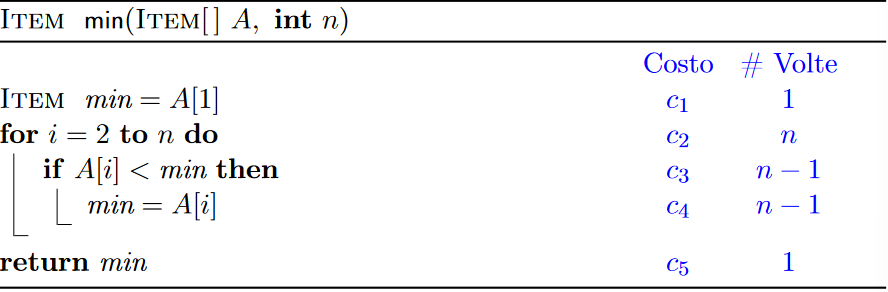
\includegraphics[width=0.9\textwidth]{01/calcoloMin.png}
            
            Otteniamo quindi che il tempo di calcolo è:
            \[
                \begin{aligned}
                    T(n)=&c_1+c_2n+c_3(n-1)+c_4(n-1)+c_5\\
                    =&(c_2+c_3+c_4)n+(c_1+c_5-c_3-c_4) = an+b
                \end{aligned}
            \]
        \subsubsection{Tempo di calcolo di $\operatorname{binarySearch}()$}
            In questo algoritmo il vettore viene suddiviso in due parti:
            $ \text{Parte SX: } \left\lfloor(n-1)/2\right\rfloor $ e $ \text{Parte DX: } \left\lfloor n/2\right\rfloor $.
            
            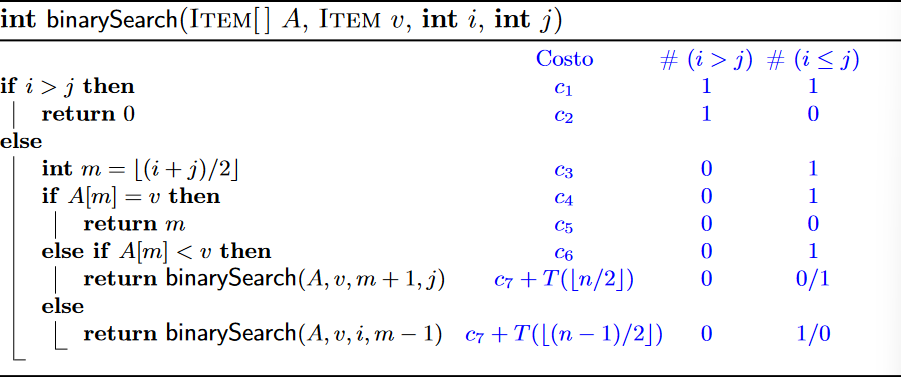
\includegraphics[width=0.9\textwidth]{01/calcoloBinarySearch.png}
            
            A questo punto dobbiamo fare delle assunzioni:
            \begin{itemize}
                \item Assumiamo che la $ n $ potenza di $ 2 $ sia: $ n = 2^k $.
                \item L'elemento cercato non è presente.
                \item Ad ogni passo andiamo sempre a destra in quanto il numero di elementi da valutare è maggiore: $ n/2 $.
            \end{itemize}
            possiamo ora suddividere il problema in due casistiche:
            $$
                \begin{aligned}
                    i>j\quad & (n=0) & T(n)=&c_1 + c_2\\
                    i\leq j\quad & (n>0) & T(n)=&T(n/2) + c_1 + c_2 + c_3 + c_4 + c_6 + c_7\\
                        &&=&T(n/2) + d
                \end{aligned}
            $$
            unendo i due casi otteniamo la \textbf{Relazione di ricorrenza}:
            $$
                T(n)=
                    \begin{cases}
                        c& \text{se } n=0\\
                        T(n/2) +d & \text{se } n>0
                    \end{cases}
            $$
            ottenuta la relazione generalmente per un numero $ n $ di elementi otteniamo che il tempo è dato da:
            $$
                \begin{aligned}
                    T(n)=&T(n/2)+d&\\
                    =&T(n/4)+2d&\\
                    &\hdots\\
                    =&T(1)+kd&\\
                    =&T(0)+(k+1)d&\\
                    =&kd+(c+d) &= d\log n + e
                \end{aligned}
            $$
            ottenendo quindi che il tempo di calcolo è $ O(\log n) $ di natura logaritmica.
    \subsection{Ordini di Complessità}
        \begin{table}[h]
            \centering
            \begin{tabular}{|c|c|c|c|c|c|}
                \hline
                $ f(n) $ & $ n=10^1 $ & $ n=10^2 $ & $n=10^3 $ & $n=10^4 $ & \textbf{Tipo} \\
                \hline
                $ \log n $ & 3 & 6 & 9 & 13 & Logaritmica \\
                \hline
                $ \sqrt{n} $ & 3 & 10 & 31 & 100 & sub-lineare \\
                \hline
                $ n $ & 10 & 100 & 1000 & 10000 & Lineare \\
                \hline
                $ n\log n $ & 30 & 664 & 9965 & 132877 & log-lineare \\
                \hline
                $ n^2 $ & $10^2$ & $10^4$ & $10^6$ & $10^8$ & Quadratica \\
                \hline
                $ n^3 $ & $10^3$ & $10^6$ & $10^9$ & $10^{12}$ & Cubica \\
                \hline
                $ 2^n $ & $1024$ & $10^{30}$ & $10^{301}$ & $10^{3010}$ & Esponenziale\\
                \hline
            \end{tabular}
        \end{table}
\section{Notazione asintotica}
\label{sec:notazioneAsintotica}
    \subsection{Notazioni \texorpdfstring{$ O $, $ \Omega $, $ \Theta $}{O, Omega, Theta}}
        \subsubsection{Notazione $ O $}
            \begin{definition}
                Sia $ g(n) $ una funzione di costo; indichiamo con $ O(g(n)) $ l'insieme delle funzioni $ f(n) $ tali per cui: 
                $$ \exists c>0,\ \exists m\geq 0: f(n) \leq cg(n),\ \forall n\geq m $$
            \end{definition}
            La seguente notazione si legge: $ f(n) $ è "O grande" (big O) di $ g(n) $, con un abuso di notazione si scrive $ f(n)=O(g(n)) $\footnote{\label{fn:note1} Questo è un abuso di notazione in quanto $ O(g(n)) $ è una classe di funzioni e non può essere eguagliata una singola funzione, il simbolo più appropriato sarebbe $ f(n)\in O(g(n)) $}
            . Inoltre per la precedente definizione possiamo dire che $ g(n) $ è un \textbf{limite asintotico superiore} per $ f(n) $, in quanto dopo qualche valore $ m $ la funzione $ g(n) $ è sempre maggiore di $ f(n) $. Inoltre per questo motivo sappiamo che $ f(n) $ cresce al più come $ g(n) $.
        \subsubsection{Notazione $ \Omega $}
            \begin{definition}
                Sia $ g(n) $ una funzione di costo; indichiamo con $ \Omega(g(n)) $ l'insieme delle funzioni $ f(n) $ tali per cui: 
                $$ \exists c>0,\ \exists m\geq 0: f(n) \geq cg(n),\ \forall n\geq m $$
            \end{definition}
            La seguente notazione si legge: $ f(n) $ è "Omega" di $ g(n) $, con un abuso di notazione si scrive $ f(n)=\Omega(g(n)) $\footref{fn:note1}. Inoltre per la precedente definizione possiamo dire che $ g(n) $ è un \textbf{limite asintotico inferiore} per $ f(n) $, in quanto dopo qualche valore $ m $ la funzione $ g(n) $ è sempre minore di $ f(n) $. Inoltre per questo motivo sappiamo che $ f(n) $ cresce almeno come $ g(n) $.
        \subsubsection{Notazione $ \Theta $}
            \begin{definition}
                Sia $ g(n) $ una funzione di costo; indichiamo con $ \Theta(g(n)) $ l'insieme delle funzioni $ f(n) $ tali per cui: 
                $$ \exists c_1>0,\ \exists c_2>0,\ \exists m\geq 0: c_1g(n) \leq f(n) \leq c_2g(n),\ \forall n\geq m $$
            \end{definition}
            La seguente notazione si legge: $ f(n) $ è "Theta" di $ g(n) $, con un abuso di notazione si scrive $ f(n)=\Theta(g(n)) $\footref{fn:note1}. Inoltre per la precedente definizione possiamo dire che $ f(n) $ cresce esattamente come $ g(n) $, detto ciò $ f(n)= \Theta(g(n)) $ se e solo se $ f(n)=O(g(n)) $ e $ f(n)=\Omega(g(n)) $.
        \subsubsection*{Esempio grafico}
            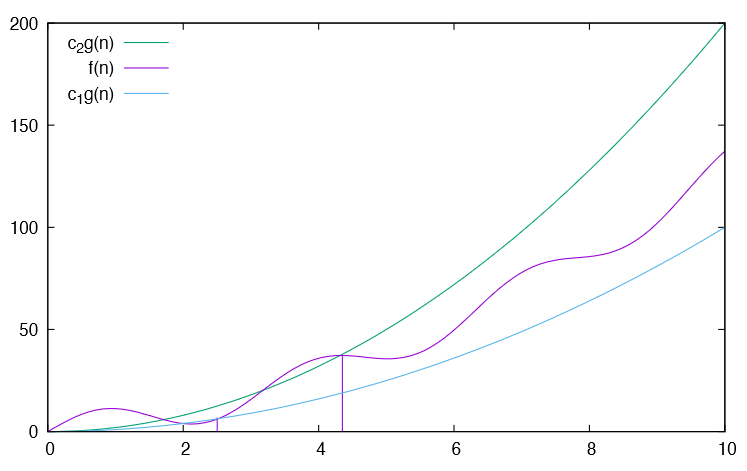
\includegraphics[width=0.5\textwidth]{01/graficoNotazioni.png}
    \subsection{Esempi e Esercizi}
        \subsubsection{Esempio 1}
            $$
                f(n) = 10n^3 + 2n^2 + 7 \stackrel{?}{=} O(n^3)
            $$
            Dobbiamo provare che $ \exists c>0,\ \exists m\geq 0: f(n) \leq cn^3,\ \forall n\geq m $.
            $$
                \begin{aligned}
                    f(n) =& 10n^3 + 2n^2 + 7\\
                    \leq & 10n^3 + 2n^3 + 7 &\quad \forall n \geq 1\\ 
                    \leq & 10n^3 + 2n^3 + n^3 &\quad  \forall n \geq \sqrt[3]{7}\\
                    = & 13 n^3 \stackrel{?}{\leq} cn^3
                \end{aligned}
            $$
            Che è verificata per qualsiasi $ c \geq 13 $ e $ m \geq \sqrt[3]{7} $, arrotondiamo $m$ ad un intero superiore ottenendo $ m = 2 $. 
            
            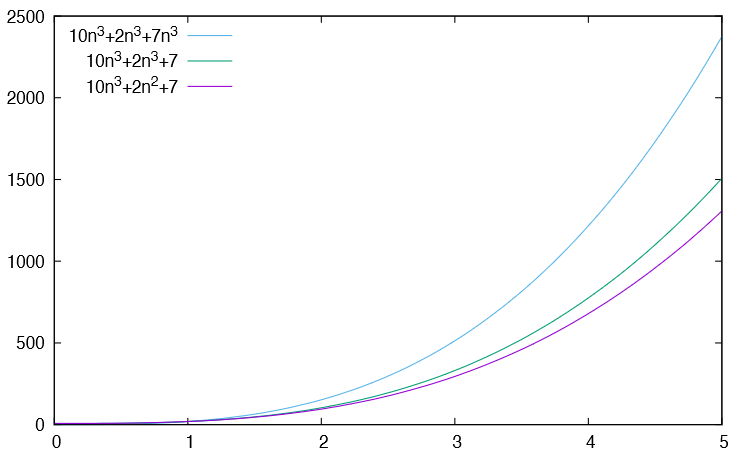
\includegraphics[width=0.5\textwidth]{01/graficoEs1.png}
\section{Complessità problemi v/s algoritmi}
    \subsection{Moltiplicazione numeri complessi}
        Per moltiplicare numeri complessi bisogna svolgere la seguente operazione:
        $$
            (a+bi)(c+di) = [ac-bd]+[ad+bc]i
        $$
        dunque dai parametri $ a,b,c,d $ otteniamo che il risultato da restituire: $ ac-bd $ e $ ad+bc $.
        \paragraph{Domande}
            Considerando che addizioni e sottrazioni costino $ c_1 = 0.01 $ e moltiplicazione costi $ c_2 = 1 $ possiamo chiederci:
            \begin{itemize}
                \item Quanto costa l'algoritmo?
                \item Si può fare meglio?
                \item Qual'è il ruolo del modello di calcolo?
            \end{itemize}
            Dato che si devono fare almeno 4 moltiplicazioni e 2 somme otteniamo che il costo totale è $ 4c_2 + 2c_1 = 4.02 $.
            
            Ora si può fare meglio? La risposta è no in quanto se si potesse fare meglio si potrebbe fare meglio allora bisognerebbe trovare un algoritmo che esegua meno di 4 moltiplicazioni e 2 somme, ma per fare ciò bisognerebbe cambiare il modello di calcolo.
    \subsection{Sommare numeri binari}
        \subsubsection{Algoritmo elementare della somma - $ \operatorname{sum}() $}
            Ipotizziamo che l'operazione da fare sia la somma di due bit singoli e generare il riporto, assegniamo a questa operazione costo $ c $.
            Dopo ciò indichiamo con $ n $ il numero massimo di bit tra i due numeri da sommare, otteniamo dunque che:
            \begin{itemize}
                \item Richiede di esaminare tutti gli $ n $ bit
                \item Costo totale $ cn = O(n) $
            \end{itemize}
        \subsubsection{Esiste allora un algoritmo più efficiente?}
            La risposta è no in quanto se esistesse un algoritmo di tale genere allora potremmo cambiare un solo bit di uno dei due numeri e ottenere un risultato diverso senza che l'algoritmo lo vada ad analizzare, il che è impossibile.
    \subsection{Moltiplicare numeri binari}
        \subsubsection{Algoritmo elementare del prodotto - $\operatorname{prod}()$}
            L'operazione elementare per moltiplicare due numeri binari è la seguente:
            $$
                \begin{array}{c c c c c c c c c c c c c c c}
                    & & & & & & & 1 & 0 & 1 & 1 & 1 & 0 & 1 & *\\
                    & & & & & & & 1 & 1 & 0 & 1 & 1 & 1 & 0 & \\
                    \hline
                    & & & & & & & 0 & 0 & 0 & 0 & 0 & 0 & 0 &\\
                    & & & & & & 1 & 0 & 1 & 1 & 1 & 0 & 1 & &\\
                    & & & & & 1 & 0 & 1 & 1 & 1 & 0 & 1 & & &\\
                    & & & & 1 & 0 & 1 & 1 & 1 & 0 & 1 & & & &\\
                    & & & 0 & 0 & 0 & 0 & 0 & 0 & 0 & & & & &\\
                    & & 1 & 0 & 1 & 1 & 1 & 0 & 1 & & & & & &\\
                    & 1 & 0 & 1 & 1 & 1 & 0 & 1 & & & & & & &\\
                    \hline
                    1 & 0 & 0 & 1 & 1 & 1 & 1 & 1 & 1 & 1 & 0 & 1 & 1 & 0\\
                \end{array}
            $$
            deduciamo che:
            \begin{itemize}
                \item Dobbiamo accedere a tutti i bit
                \item Il costo totale è $ cn^2 = O(n^2) $ perché dobbiamo fare $ n $ somme di $ n $ bit.
            \end{itemize}
        \subsubsection{Soluzione Divide-et-impera}
            La base del principio \textbf{Divide-et-impera} è la seguente:
            \begin{description}
                \item[Divide] Dividere il problema in sotto-problemi più piccoli.
                \item[Impera] risolvi i sotto-problemi in modo ricorsivo.
                \item[Combina] combina le soluzioni dei sotto-problemi per ottenere la soluzione del problema originale.  
            \end{description}
            La soluzione divide-et-impera per il problema della moltiplicazione binaria è la seguente:
            $$
                \begin{aligned}
                    \begin{aligned}
                        X=& a\cdot 2^{n/2} + b\\
                        Y=& c\cdot 2^{n/2} + d\\
                        XY =& ac\cdot 2^n + (ad+bc)\cdot 2^{n/2} + bd
                    \end{aligned}
                    &\quad
                    \begin{aligned}
                        X &= \stackrel{a}{\text{Parte SX}}\quad \stackrel{b}{\text{Parte DX}}\\
                        Y &= \stackrel{c}{\text{Parte SX}}\quad \stackrel{d}{\text{Parte DX}}
                    \end{aligned}
                \end{aligned}
            $$
            Ora possiamo scrivere l'algoritmo:
            \begin{algorithm}
                \caption{boolean[ ] pdi(boolean[ ] X, boolean[ ] Y, int n)}\label{alg:pdi}
                \begin{algorithmic}[1]
                    \If{$n=1$}
                        \State \Return $X[1]\cdot Y[1]$
                    \Else
                        \State spezza $X$ in $a$ e $b$ e $Y$ in $c$ e $d$
                        \State \Return pdi($a,c,n/2$)$\cdot 2^n$ + (pdi($a,d,n/2$) + pdi($b,c,n/2$))$\cdot 2^{n/2}$ + pdi($b,d,n/2$)
                    \EndIf
                \end{algorithmic}
            \end{algorithm}
            La funzione di costo associata all'algoritmo è:
            $$
                T(n)=\begin{cases}
                    c_1 & n=1\\
                    4T(n/2)+c_2\cdot n &  n>1
                \end{cases}
            $$
            \textbf{Nota:} moltiplicare per $2^n$ corrisponde a uno shift a sinistra di $n$ posizioni, svolta in tempo lineare.

            Ora in quanto abbiamo $ 4 $ chiamate ricorsive, assumendo che $c_1$ sia il tempo per moltiplicare due bit e che $ c_2 $ sia il tempo per sommare due numeri binari otteniamo che il tempo di calcolo è $ c_2 \cdot 4^i \cdot \frac{n}{2^i} = T(1) \cdot 4^{\log_2 n} = c_1 \cdot n^{\log_2 4} = c_1 \cdot n^2 $.
            \subparagraph{Ma allora è possibile fare meglio?}
            Long story short: si in quanto è stato provato nel 2021 l'esistenza di un algoritmo di complessità $ O(n\log n) $. 
\section{Algoritmi di Ordinamento}
    \paragraph{Introduzione} L'obbiettivo di questa sezione è valutare la complessità degli algoritmi in base all'input, in alcuni casi gli algoritmi si comportano differentemente in base all'input se siamo a conoscenza dell'input questa ci consente di scegliere un algoritmo più adeguato alla nostra soluzione.
    \paragraph{Come analiziamo gli algoritmi}
        Possiamo analizzare l'efficienza degli algoritmi in base a diversi casi:
        \subparagraph{Caso Pessimo}
            Questa analisi è la più importante in quanto sappiamo che questa restituisce il limite superiore al tempo di esecuzione qualsiasi sia l'input.
        \subparagraph{Caso Medio}
            Questa analisi è la più complessa in quanto bisogna definire il "caso medio" e cosa si intende per "medio", ma è utile con una distribuzione uniforme degli input.
        \subparagraph{Caso Ottimo}
            Utile solo se conosciamo qualcosa sull'input, altrimenti non risulta utile se abbiamo un input arbitrario.
    \subsection{Selection Sort}
        Algoritmo Selection Sort:
        \begin{algorithm}
            \caption{selectionSort(Item[ ] A, \Int n)}\label{alg:selectionSort}
            \begin{algorithmic}[1]
                \For{$i=1$ \To $n-1$}
                    \State \Int $min \gets \operatorname{min}(A,i,n)$
                    \State $A[i]$ $\leftrightarrow$ $\operatorname{min}(A,i,n) $
                \EndFor
            \end{algorithmic}
        \end{algorithm}

        Algoritmo di supporto min:
        \begin{algorithm}
            \caption{int min(Item[ ] A, \Int i, \Int n)}\label{alg:min}
            \begin{algorithmic}[1]
                \State \Int min $\gets i$
                \For{$j=i+1$ \To $n$}
                    \If{$A[j]<A[min]$}
                        \State min $\gets j$
                    \EndIf
                \EndFor
                \State \Return min
            \end{algorithmic}
        \end{algorithm}
        Avendo analizzato il seguente algoritmo notiamo come in ogni caso, ottimo, medio e pessimo, il "ciclo" esterno della funzione $ \operatorname{selectionSort}() $ viene eseguito $ n-1 $ volte, mentre il ciclo interno della funzione $ \operatorname{min}() $ viene eseguito $ n-i $ dove $ i $ è il valore dell'iterazione del ciclo esterno, quindi $ n-1 + n-2 + n-3 + \ldots + 1 = \frac{n(n-1)}{2} $ volte, otteniamo quindi che il tempo di calcolo è $ O(n^2) $ in quanto questo si può approssimare a $ \frac{n^2}{2} $.
        $$  
            \sum_{i=1}^{n-1} n-i = \sum_{i=1}^{n-1} i = \frac{n(n-1)}{2}= O(n^2)
        $$
    \subsection{Insertion Sort}
        L'algoritmo di insertion sort è efficiente per ordinare piccoli insiemi, il concetto dietro a questo si bassa sull'inserimento dell'elemento preso in analisi al posto giusto.
        
        Algoritmo Insertion Sort:
        \begin{algorithm}
            \caption{insertionSort(Item[ ] A, \Int n)}\label{alg:insertionSort}
            \begin{algorithmic}[1]
                \For{$i=2$ \To $n$}
                    \State Item $temp \gets A[i]$
                    \State \Int $j \gets i$
                    \While{$j>1$ and $A[j-1]>temp$}
                        \State $A[j] \gets A[j-1]$
                        \State $j \gets j-1$
                    \EndWhile
                    \State $A[j] \gets temp$
                \EndFor
            \end{algorithmic}
        \end{algorithm}
        
        Il costo di esecuzione non dipende esclusivamente dalla dimensione ma anche dall'ordine degli elementi in ingresso.
        \subparagraph{Caso Pessimo} Il costo dunque nel \textbf{caso pessimo} è $ O(n^2) $ in quanto vengono eseguiti $ n-1 $ cicli esterni e $ n-1 $ cicli interni, ottenendo dunque $ (n-1) + (n-2) + \ldots + 1 = \frac{n(n-1)}{2} = O(n^2) $.
        \subparagraph{Caso Medio }Nel \textbf{caso medio} il costo rimane $ O(n^2) $ in quanto il ciclo interni viene eseguito $ n/2 $ volte, ottenendo dunque $ \frac{n(n-1)}{4} = O(n^2) $.
        \subparagraph{Caso Ottimo} Nel \textbf{caso ottimo} il costo è $ O(n) $ in quanto il ciclo interno non viene mai eseguito.
        
        Questo ci porta a dire che il $ \operatorname{insertionSort}() $ è un algoritmo di ordinamento utile nei casi in cui l'input è già ordinato o quasi ordinato, nei casi nei quali non conosciamo la natura dell'input è meglio utilizzare un algoritmo di ordinamento differente.
    \subsection{Merge Sort}
        L'algoritmo di $ \operatorname{mergeSort}() $ è un algoritmo di ordinamento basato sul principio \textbf{divide-et-impera}.
        \begin{description}
            \item[Divide:] Spezza virtualmente il vettore di $ n $ elementi in sotto-vettori di $ n/2 $ elementi.
            \item[Impera:] Chiama $ \operatorname{mergeSort}() $ ricorsivamente sui due sotto-vettori.
            \item[Combina:] Unisci (\textbf{merge}) i due sotto-vettori ordinati in un unico vettore ordinato. 
        \end{description}
        In input si ha:
        \begin{itemize}
            \item $ A $: vettore di $ n $ elementi.
            \item $ \text{start}, \text{end}, \text{mid} $ sono tali che $ 1\leq \text{start} < \text{mid} < \text{end} \leq n $.
            \item I sotto-vettori $ A[\text{start},\ldots,\text{mid}] $ e $ A[\text{mid}+1,\ldots,\text{end}] $ sono ordinati.
        \end{itemize}
        In output si hanno i due sotto-vettori fusi in un unico sotto-vettore ordinato, tramite un vettore di appoggio $ B $.

        Funzione di appoggio $\operatorname{Merge}$:
        \begin{algorithm}
            \caption{Merge(Item[ ] A, \Int start, \Int end, \Int mid)}\label{alg:merge}
            \begin{algorithmic}[1]
                \State \Int $i,j,k,h$
                \State \Int $i \gets \text{start}$
                \State \Int $j \gets \text{mid}+1$
                \State \Int $k \gets \text{start}$
                \While {$i \leq \text{mid}$ and $j \leq \text{end}$}
                    \If{$A[i] \leq A[j]$}
                        \State $B[k] \gets A[i]$
                        \State $i \gets i+1$
                    \Else
                        \State $B[k] \gets A[j]$
                        \State $j \gets j+1$
                    \EndIf
                    \State $k \gets k+1$
                \EndWhile
                \State $j \gets \text{end}$
                \For {$h=\text{mid}$ \DownTo $i$}
                    \State $A[j] \gets A[h]$
                    \State $j \gets j-1$
                \EndFor
                \For {$j=\text{start}$ \To $k-1$}
                    \State $A[j] \gets B[j]$
                \EndFor
            \end{algorithmic}
        \end{algorithm}
        
        Il costo computazionale di $ \operatorname{Merge}() $ è $ O(n) $, questa è la base del costo computazionale di $ \operatorname{mergeSort}() $.
        \newpage % Usato per evitare che l'algoritmo venga spezzato tra due pagine diverse
        Funzione completa $ \operatorname{mergeSort}() $:

        \begin{algorithm}
            \caption{mergeSort(Item[ ] A, \Int start, \Int end)}\label{alg:mergeSort}
            \begin{algorithmic}[1]
                \If{$\text{start}<\text{end}$}
                    \State \Int $mid \gets (\text{start}+\text{end})/2$
                    \State mergeSort($A,\text{start},\text{mid}$)
                    \State mergeSort($A,\text{mid}+1,\text{end}$)
                    \State merge($A,\text{start},\text{end},\text{mid}$)
                \EndIf
            \end{algorithmic}
        \end{algorithm}

        Assumendo per semplificare che $ n = 2^k $ dove $ k $ è un intero allora l'altezza dell'albero è esattamente $ k = \log n $, in questo modo tutti i sotto-vettori hanno dimensione che è potenza di 2.
        Così facendo il costo computazionale di $ \operatorname{mergeSort}() $ è:
        $$
            T(n)=\begin{cases}
                c & n=1\\
                2T(n/2)+dn & n>1
            \end{cases}
        $$
        dove $ c $ è il costo di un'operazione elementare, $ d $ è il costo di $ \operatorname{Merge}() $ e $ n $ è il costo di copiare i valori da $ B $ a $ A $.
    \chapter{Analisi di funzioni}
\thispagestyle{chapterInit}
\section{Notazione asintotica}
    \subsection{Definizioni}
        Si rimanda al \hyperref[sec:notazioneAsintotica]{sezione 1.2} per le definizioni di $O$, $\Omega$ e $\Theta$.
\section{Proprietà della notazione asintotica}
    \subsection{Regola Generale}
        Da qui si prende in considerazione la seguente espressione polinomiale:
        $$
            f(n) = a_kn^k + a_{k-1}n^{k-1} + \ldots + a_1n + a_0, \quad a_k > 0 \Rightarrow f(n) = \Theta(n^k)
        $$
        \paragraph{Limite Superiore} $ \exists c>0, \exists m\geq 0: f(n)\leq cn^k,\forall n\geq m $
            $$
                \begin{aligned}
                    f(n)=&a_kn^k + a_{k-1}n^{k-1} + \ldots + a_1n + a_0 \\
                    \leq& a_kn^k + \left|a_{k-1}\right|n^{k-1} + \ldots + \left|a_1\right|n + \left|a_0\right| \\
                    \leq& a_kn^k + \left|a_{k-1}\right|n^k + \ldots + \left|a_1\right|n^k + \left|a_0\right|n^k \\
                    =& (a_k + \left|a_{k-1}\right| + \ldots + \left|a_1\right| + \left|a_0\right|)n^k \quad& \forall n\geq 1\\
                    \stackrel{?}{\leq}& cn^k
                \end{aligned}
            $$
            questa è vera per $ c\geq \left(a_k + \left|a_{k-1}\right| + \ldots + \left|a_1\right| + \left|a_0\right| \right) >0$ e per $m=1$
        \paragraph{Limite Inferiore} $ \exists d > 0, \exists m\geq 0: f(n)\geq dn^k,\forall n\geq m $
            $$
                \begin{aligned}
                    f(n)=&a_kn^k + a_{k-1}n^{k-1} + \ldots + a_1n + a_0 \\
                    \geq& a_kn^k - \left|a_{k-1}\right|n^{k-1} - \ldots - \left|a_1\right|n - \left|a_0\right| \\
                    \geq& a_kn^k - \left|a_{k-1}\right|n^k - \ldots - \left|a_1\right|n^k - \left|a_0\right|n^k \\
                    =& (a_k - \left|a_{k-1}\right| - \ldots - \left|a_1\right| - \left|a_0\right|)n^k \quad& \forall n\geq 1\\
                    \stackrel{?}{\geq}& dn^k
                \end{aligned}
            $$
            questa è vera se: $ d\leq a_k - \frac{\left|a_{k-1}\right|}{n} - \ldots - \frac{\left|a_1\right|}{n} - \frac{\left|a_0\right|}{n} >0 \Leftrightarrow n>\frac{\left|a_{k-1}\right| + \ldots + \left|a_1\right| + \left|a_0\right|}{a_k} $     
        \subsubsection{Casi Particolari}
            \paragraph{Complessità di $ f(n) = 5 $}
                $$
                    \begin{aligned}
                        f(n) = 5 \geq c_1n^0 \Rightarrow c_1\leq 5 \\
                        f(n) = 5 \leq c_2n^0 \Rightarrow c_2\geq 5 \\
                        \Rightarrow f(n) = \Theta(n^0) = \Theta(1)
                    \end{aligned}
                $$
            \paragraph{Complessità di $ f(n) = 5 + \sin(n) $}
                La complessità di calcolo di $ f(n) $ è $ \Theta(1) $, in quanto $ \sin(n) $ è una funzione oscillante tra $ -1 $ e $ 1 $, quindi $ 5 + \sin(n) $ oscilla tra $ 4 $ e $ 6 $.

                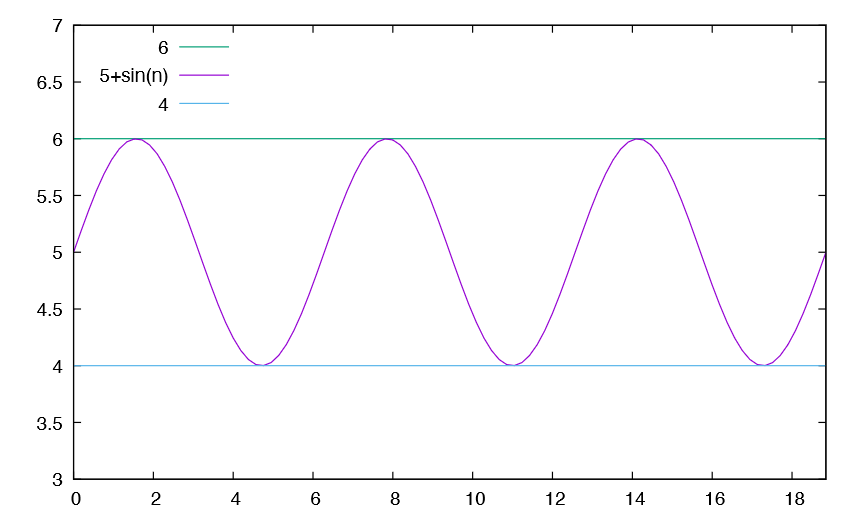
\includegraphics[scale=0.5]{02/graficoFsin.png}
    \subsection{Proprietà delle notazioni}
        \subsubsection{Dualità}
            $ f(n) = O(g(n)) \Leftrightarrow g(n) = \Omega(f(n)) $
            \begin{proof}
                $$
                    \begin{aligned}
                        f(n) = O(g(n)) \Leftrightarrow & f(n) \leq cg(n), \forall n\geq m \\
                        \Leftrightarrow & g(n) \geq \frac1cf(n), \forall n\geq m \\
                        \Leftrightarrow & g(n) \geq c'f(n), \forall n\geq m, c'=\frac1c \\
                        \Leftrightarrow & g(n) = \Omega(f(n))
                    \end{aligned}
                $$
            \end{proof}
        \subsubsection{Eliminazione di costanti}
            $$
                \begin{aligned}
                    f(n) &= O(g(n)) \Leftrightarrow af(n)=O(g(n)), \forall a>0 \\
                    f(n) &= \Omega(g(n)) \Leftrightarrow af(n)=\Omega(g(n)), \forall a>0 \\
                \end{aligned}
            $$
            \begin{proof}                
                $$
                    \begin{aligned}
                        f(n)=O(g(n)) \Leftrightarrow & f(n)\leq cg(n), \forall n\geq m \\
                        \Leftrightarrow & af(n)\leq acg(n), \forall n\geq m,\forall a>0 \\
                        \Leftrightarrow & af(n)\leq c'g(n), \forall n\geq m,c'=ac>0 \\
                        \Leftrightarrow & af(n)=O(g(n)), \forall a>0
                    \end{aligned}
                $$
            \end{proof}
        \subsubsection{Sommatoria (sequenza di algoritmi)}
            $$
                \begin{aligned}
                    f_1(n) = O(g_1(n)), f_2(n) = O(g_2(n)) \Rightarrow f_1(n) + f_2(n) = O(\max(g_1(n),g_2(n)))\\
                    f_1(n) = \Omega(g_1(n)), f_2(n) = \Omega(g_2(n)) \Rightarrow f_1(n) + f_2(n) = \Omega(\max(g_1(n),g_2(n)))
                \end{aligned}
            $$
            \begin{proof}[Dimostrazione (Lato $ O $).]
                $$
                    \begin{aligned}
                        f_1(n) = O(g_1(n)) \land f_2(n) = O(g_2(n)) & \Rightarrow \\
                        f_1(n) \leq c_1g_1(n) \land f_2(n) \leq c_2g_2(n) & \Rightarrow \\
                        f_1(n) + f_2(n) \leq c_1g_1(n) + c_2g_2(n) & \Rightarrow \\
                        f_1(n) + f_2(n) \leq \max\{c_1,c_2\}(2\cdot \max(g_1(n),g_2(n))) & \Rightarrow \\
                        f_1(n) + f_2(n) = O(\max(g_1(n),g_2(n))) &
                    \end{aligned}
                $$
            \end{proof}
        \subsubsection{Prodotto (cicli annidati)}
            $$
                \begin{aligned}
                    f_1(n) = O(g_1(n)), f_2(n) = O(g_2(n)) \Rightarrow f_1(n) \cdot f_2(n) = O(g_1(n) \cdot g_2(n))\\
                    f_1(n) = \Omega(g_1(n)), f_2(n) = \Omega(g_2(n)) \Rightarrow f_1(n) \cdot f_2(n) = \Omega(g_1(n) \cdot g_2(n))
                \end{aligned}
            $$
            \begin{proof}
                $$
                    \begin{aligned}
                        f_1(n) = O(g_1(n)) \land f_2(n) = O(g_2(n)) & \Rightarrow \\
                        f_1(n) \leq c_1g_1(n) \land f_2(n) \leq c_2g_2(n) & \Rightarrow \\
                        f_1(n)\cdot f_2(n) \leq c_1c_2g_1(n)g_2(n) &
                    \end{aligned}
                $$
        \end{proof}
        \subsubsection{Simmetria}
            $$
                f(n) = \Theta(g(n)) \Leftrightarrow g(n) = \Theta(f(n))
            $$
            \begin{proof}
                Grazie alla proprietà della dualità, si ha che:
                $$
                    \begin{aligned}
                        f(n) = \Theta(g(n)) &\quad \Rightarrow \quad f(n) = O(g(n)) \Rightarrow g(n) = \Omega(f(n))\\
                        f(n) = \Theta(g(n)) &\quad \Rightarrow \quad f(n) = \Omega(g(n)) \Rightarrow g(n) = O(f(n))
                    \end{aligned}
                $$
            \end{proof}
        \subsubsection{Transitività}
            $$
                \begin{aligned}
                    f(n) = O(g(n)), g(n) = O(h(n)) \Rightarrow f(n) = O(h(n))
                \end{aligned}
            $$
            \begin{proof}
                $$
                    \begin{aligned}
                        f(n) = O(g(n)) \land g(n) = O(h(n)) & \Rightarrow \\
                        f(n) \leq c_1g(n) \land g(n) \leq c_2h(n) & \Rightarrow \\
                        f(n) \leq c_1c_2h(n) & \Rightarrow \\
                        f(n) = O(h(n)) &
                    \end{aligned}
                $$
            \end{proof}
    \subsection{Altre funzioni di costo}
        \subsubsection{Logaritmi v/s funzioni lineari}
            \paragraph{Proprietà dei Logaritmi}
                Vogliamo provare che $ \log(n) = O(n) $. Dimostriamo per induzione che
                $$
                    \exists c>0,\exists m\geq 0:\log n\leq cn,\forall n\geq m\qquad \text{definizione di }O
                $$
                \begin{proof}
                    \begin{basecase} ($ n=1 $):
                        $ \log 1 = 0 \leq \stackrel{c}0\cdot \stackrel{n}1 = 0 $
                    \end{basecase}
                    \textbf{Ipotesi induttiva}: sia $ \log k \leq ck, \forall k\leq n $.
                    \begin{inductivecase}
                        Dimostriamo la proprietà per $ n+1 $:
                        $$
                            \begin{aligned}
                                \log(n+1) \leq & \log(n+n) = \log 2n & \forall n\geq 1 \\
                                = & \log 2 + \log n \qquad & \log ab = \log a + \log b \\
                                = & 1 + \log n & \log 2 = 1 \\
                                \leq & 1 + cn & \text{per induzione} \\
                                \stackrel{?}{\leq} & c(n+1) & \text{Obbiettivo} \\
                                1+cn\leq c(n+1) \Leftrightarrow & c\geq 1
                            \end{aligned}
                        $$
                    \end{inductivecase}
                \end{proof}
        \subsection{Giocando con le espressioni}
            \paragraph{Es 1}
                È vero che $ \log_a n = \Theta(\log n) $?

                Si: $ \log_a n = (\log_a 2) \cdot (\log_2 n) = \Theta(\log n) $
            
            \paragraph{Es 2}
                È vero che $ \log n^a = \Theta(\log n) $, per $ a>0 $?

                Si: $ \log n^a = a\log n = \Theta(\log n) $
            
            \paragraph{Es 3}
                È vero che $ 2^{n+1} = \Theta(2^n) $?

                Si: $ 2^{n+1} = 2\cdot 2^n = \Theta(2^n) $
            \paragraph{Es 4}    
                È vero che $ 2^{n} = \Theta(3^n) $?

                Ovviamente $ 2^{n} = O(3^n) $

                Ma: $ 3^{n} = \left(\frac32\cdot 2\right)^n=\left(\frac32\right)^n\cdot 2^n: $ Quindi non esiste $ c > 0 $ tale per cui $ \left(\frac32\right)^n\cdot 2^n\leq c2^n $, quindi $ 2^n \neq O(3^n) $
    \subsection{Classificazione delle funzioni}
        È possibile definire un ordinamento delle principali classi estendendo le relazioni che abbiamo dimostrato:
        
        Per ogni $r<s,h<k,a<b$:
        $$
            o(1) \subset O(\log^r n) \subset O(\log^s n) \subset O(n^h) \subset O(n^h \log^r n ) \subset O(n^h \log^s n) \subset O(n^k) \subset O(a^n) \subset O(b^n)
        $$
\section{Ricorrenze}
    \subsection{Introduzione}
        \paragraph{Equazioni di ricorrenza} Quando si calcola la complessità di un algoritmo ricorsivo, questa viene espressa tramite un'\textbf{equazione di ricorrenza}, ovvero una formula definita in maniera ricorsiva.
            \subparagraph{MergeSort}
                $$
                    T(n) = \begin{cases}
                        1 & \text{se } n=1 \\
                        2T\left(\frac{n}{2}\right) + n & \text{se } n>1
                    \end{cases}
                $$
        \paragraph{Forma Chiusa} L'obbiettivo è quello di ottenere, quando possibile, una \textbf{formula chiusa} che rappresenti la classe di complessità della funzione.
            \subparagraph{MergeSort}
                $$ 
                    T(n) = \begin{cases}
                        T(\lfloor n/2 \rfloor) + T(\lceil n/2 \rceil) + \Theta(n) & n > 1 \\
                        \Theta(1) & n \leq 1
                    \end{cases} \Longrightarrow T(n) = \Theta(n\log n)
                $$
    \subsection{Metodo dell'albero di ricorsione, o per livelli}
        \paragraph{Introduzione} "Srotoliamo" la ricorrenza in un albero i costi ai vari livelli della ricorsione.
        \subsubsection{Esempio 1}
            $$
                T(n)=\begin{cases}
                    T(n/2) + b & n>1 \\
                    c & n\leq 1
                \end{cases}
            $$
            È possibile risolvere questa ricorrenza nel modo seguente:
            $$
                \begin{aligned}
                    T(n) = & b + T(n/2) \\
                    = & b + b + T(n/4) \\
                    = & b + b + b + T(n/8) \\
                    = & \ldots \\
                    = & \underbrace{b+b+\ldots+b}_{\log n} + T(1) \\
                \end{aligned}
            $$
            Assumiamo per semplicità che $ n=2^k $. $ T(n) = b\log n + c = \Theta(\log n) $
        \subsubsection{Esempio 2}
            $$
                T(n)=\begin{cases}
                    4T(n/2) + n & n>1 \\
                    1 & n\leq 1
                \end{cases}
            $$
            È possibile risolvere questa ricorrenza nel modo seguente:
            $$
                \begin{aligned}
                    T(n)=&\cancel{n\sum_{j=0}^{\log(n-1)} 2^j} &\underbrace{+4^{\log n}}_{\text{somma degli }T(1)}\\
                    \Rightarrow &\underbrace{n\cdot \frac{\overbrace{2^{\log n }}^{n\text{ per prop. log.}}-1}{2-1}}_{\stackrel{\text{usando: }}{\forall x\neq 1:\sum_{j=0}^kx^j=\frac{x^{k+1}-1}{x-1}}}&+4^{\log n}\\
                    =& n(n-1)&+4^{\log n}\\
                    =& n^2-n&\overbrace{+n^2}^{\text{cambiamento di base}}\\
                    =& 2n^2-n = \Theta(n^2)
                \end{aligned}
            $$
        \subsubsection{Esempio 3}
        $$
            T(n)=\begin{cases} 4T(n/2) + n^3 & n>1 \\ 1 & n\leq 1 \end{cases}
        $$
        Da questa equazione notiamo che il primo livello ha costo $ n^3 $, il secondo $ 4\left(\frac{n}{2}\right)^3 $ il terzo $ 4^2\left(\frac{n}{2^2}\right)^3 $ e così via. Quindi possiamo scrivere la sommatoria:
        $$
            \begin{aligned}
                T(n)=& n^3 + 4\left(\frac{n}{2}\right)^3 + \ldots + 4^{\log n-1}\left(\frac{n}{2^{\log n-1}}\right)^3 &+ 4^{\log n} \\
                =& \sum_{i=0}^{\log n-1}4^i\left(\frac{n}{2^i}\right)^3 & + 4^{\log n} \\
                =& n^3\sum_{i=0}^{\log n-1}\left(\frac{2^{2i}}{2^{3i}}\right) & + 4^{\log n} \\
                =& n^3\sum_{i=0}^{\log n-1}\left(2^{2i-3i}\right) & + 4^{\log n} \\
                =& n^3\sum_{i=0}^{\log n-1}\left(2^{-1\cdot i}\right) & + 4^{\log n} \\
                =& n^3\sum_{i=0}^{\log n-1}\left(\frac{1}{2}\right)^i & \overbrace{+n^2}^{\text{cambiamento di base}} \\
                \leq & n^3\sum_{i=0}^{\infty}\left(\frac{1}{2}\right)^i & +n^2 \\
                =& n^3\cdot \overbrace{\frac{1}{1-\frac{1}{2}}}^{\text{usando: }\forall x,|x|\leq 1:\sum_{i=0}^{\infty}x^i=\frac{1}{1-x}} & +n^2 \\
                =& 2n^3 + n^2
            \end{aligned}
        $$
        \footnote{In quanto la sommatoria tende a crescere allora abbiamo potuto sostituire $ \log n $ con $ \infty $ e modificare il segno di uguaglianza con quello di $ \leq $ in quanto la sommatoria verso l'infinito converge è più grande di quella finita}\newline
        Abbiamo dunque dimostrato che $ T(n) \leq 2n^3 + n^2 = O(n^3) $ però non possiamo, tramite la dimostrazione precedente, dire che $ T(n) = \Theta(n^3) $ in quanto siamo passati ad una disequazione. In questo particolare caso d'altra parte possiamo notare che $ T(n) \geq n^3 $ il che ci porta ad affermare che $ T(n) = \Omega(n^3) $ e quindi $ T(n) = \Theta(n^3) $. 
    \subsection{Metodo di sostituzione}
        \paragraph{Introduzione} È il metodo in cui si cerca di \textbf{indovinare} (\textbf{guess}) la soluzione e si prova a dimostrarla per \textbf{induzione}.
        \subsubsection{Primo esempio}
            $$ T(n) = \begin{cases} T(\lfloor n/2 \rfloor) + n & n>1 \\ 1 & n\leq 1 \end{cases} $$
            Notiamo come il costo dei vali livelli sia $ n + n/2 + n/4 + \ldots $. Dunque possiamo ipotizzare di poter scrivere:
            $$
                \begin{aligned}
                    T(n)=& n \cdot \sum_{i=0}^{\log n}\left(\frac{1}{2}\right)^i\\
                    \leq & n \cdot \sum_{i=0}^{\infty}\left(\frac{1}{2}\right)^i\\
                    = & n \cdot \underbrace{\frac{1}{1-\frac{1}{2}}}_{\text{usando }\forall x,|x| < 1: \sum_{i=0}^{\infty}x^i=\frac{1}{1-x}}\\
                    = & 2n
                \end{aligned}
            $$
            \footnote{Abbiamo potuto usare il $ \leq $ in quanto la sommatoria in questione all'infinito è sempre maggiore di quella finita e ci stiamo calcolando il costo massimo}
            \paragraph{Limite superiore}
                Tentiamo quindi ora di dire che $ T(n) = O(n) $:
                \subparagraph{Caso Base} $ T(1) = 1 \stackrel{?}{\leq} 1 \cdot c \Leftrightarrow \forall c\geq 1 $
                \subparagraph{Passo Induttivo} Dimostriamo la disequazione per $T(n)$
                $$
                    \begin{aligned}
                        T(n) = & T(\lfloor n/2 \rfloor) + n \\
                        \leq & \overbrace{c\lfloor n/2 \rfloor}^{\text{ipotizzato} O(n)} + n \\
                        \leq & c\cdot\overbrace{n/2}^{\text{intero inferiore}} + n \\
                        = & n(c/2 + 1) \\
                        \stackrel{?}{\leq} & cn \\
                        \Leftrightarrow & c/2 + 1 \leq c \Leftrightarrow c\geq 2
                    \end{aligned}
                $$
                
                Dunque abbiamo provato che: $ T(n) \leq cn $, nel caso base $ c\geq 1 $ e nel passo induttivo $ c\geq 2 $. In quanto deve valere per entrambi i casi allora il primo valore utile di $ c $ è $2$, avendo provato che per $ n=1 $ la disequazione vale e che per tutti i successivi valori di $ n $ la disequazione vale allora possiamo dire che $ T(n) = O(n) $.
            \paragraph{Limite Inferiore}
                Tentiamo di dimostrare che $ T(n) = \Omega(n) $:
                \subparagraph{Caso Base} Dimostriamo che $ T(1) = 1 \stackrel{?}{\geq} 1\cdot d \Leftrightarrow \forall d\leq 1 $
                \newpage % Per evitare che il passo induttivo vada a capo
                \subparagraph{Passo Induttivo} Dimostriamo la disequazione per $ T(n) $:
                $$
                    \begin{aligned}
                        T(n) =& T(\lfloor n/2 \rfloor) + n \\
                        \geq & \overbrace{d\lfloor n/2 \rfloor}^{\text{per ipo. induttiva sostituzione}} + n \\
                        \geq & d\cdot\overbrace{\frac{n}2-1}^{\text{intero inferiore}} + n \\
                        = & \left(\frac{d}2-\frac1n+1\right)n \stackrel{?}{\geq} dn \\
                        \Leftrightarrow & \frac{d}2-\frac1n+1 \geq d \\ 
                        \Leftrightarrow & d\leq 2 - \frac2n
                    \end{aligned}
                $$

                Abbiamo quindi dimostrato che $ T(n) \geq dn $, nel caso base $ d\leq 1 $ e nel passo induttivo $ d\leq 2 - \frac2n $. In quanto deve valere per entrambi i casi allora il primo valore utile di $ d $ è $1$, avendo provato che per $ n=1 $ la disequazione vale e che per tutti i successivi valori di $ n $ la disequazione vale allora possiamo dire che $ T(n) = \Omega(n) $.
                
            \paragraph{Conclusione} Avendo provato che $ T(n) = O(n) $ e $ T(n) = \Omega(n) $ e ricordando che se $ T(n) = O(n) \land T(n) = \Omega(n) \Leftrightarrow T(n) = \Theta(n) $ concludendo che la funzione di costo di $ T(n) $ cresce in maniera lineare.
        \subsubsection{Terzo esempio - Difficoltà matematiche}
            $$
                T(n)=\begin{cases} T\left(\left\lfloor\frac{n}2\right\rfloor\right) + T\left(\left\lceil\frac{n}2\right\rceil\right) + 1 & n>1 \\ 1 & n\leq 1 \end{cases}
            $$
            \paragraph{Limite Superiore}
                Dalla seguente si può notare come il costo di ogni livello sia $ 1 $ e che il numero di livelli sia $ \log n $. Inoltre la ricorsione viene eseguita su due rami, quindi possiamo scrivere la seguente sommatoria:
                $$
                    \begin{aligned}
                        T(n)=&\sum_{i=0}^{\log n}2^i\\
                        =&1+2+4+\ldots+\frac{n}4+\frac{n}2+n \\
                        =&O(n)
                    \end{aligned}
                $$
                Proviamo ora a dimostrare che $ T(n) = O(n) $:
                \subparagraph{Passo Induttivo} Ipotizzando che $ \forall k<n:T(k)\leq ck $, dimostriamo che $ T(n)\leq cn $:
                    $$
                        \begin{aligned}
                            T(n)=&T\left(\left\lfloor\frac{n}2\right\rfloor\right) + T\left(\left\lceil\frac{n}2\right\rceil\right) + 1 \\
                            \leq & c\left\lfloor\frac{n}2\right\rfloor + c\left\lceil\frac{n}2\right\rceil + 1 \\
                            \leq & cn+1 \\
                            \stackrel{?}{\geq} & cn \Rightarrow 1\leq 0 & \text{ impossibile}
                        \end{aligned}
                    $$
                    Sebbene la dimostrazione sia fallita ma l'intuizione ci dice che $ T(n) = O(n) $

                Proviamo dunque a dimostrarlo per un \textbf{ordine inferiore}: $ cn+1\leq cn $
                \subparagraph{Passo Induttivo} Ipotizzando che $ \exists b>0,\forall k<n:T(k)\leq ck-b $ allora dimostriamo la disequazione per $T(n)$:
                    $$
                        \begin{aligned}
                            T(n)=&T\left(\left\lfloor\frac{n}2\right\rfloor\right) + T\left(\left\lceil\frac{n}2\right\rceil\right) + 1 \\
                            \leq & c\left\lfloor\frac{n}2\right\rfloor - b + c\left\lceil\frac{n}2\right\rceil - b + 1 \\
                            =& cn - 2b + 1 \\
                            \stackrel{?}{\leq} & cn - b \\
                            \Rightarrow & \cancel{cn} - 2b + 1 \leq \cancel{cn} - b \Rightarrow b\geq 1
                        \end{aligned}
                    $$
                    Dimostriamo il passo base per $ b=1 $: $ T(1) = 1 \stackrel{?}{\leq} 1\cdot c - b\Leftrightarrow \forall c\geq b+1 $
            \paragraph{Limite Inferiore} 
                Proviamo ora a dimostrare che $ T(n) = \Omega(n) $:
                \subparagraph{Passo Induttivo} Ipotizzando che $ \forall k<n:T(k)\geq dk $, dimostriamo che $ T(n)\geq dn $:
                    $$
                        \begin{aligned}
                            T(n)=&T\left(\left\lfloor\frac{n}2\right\rfloor\right) + T\left(\left\lceil\frac{n}2\right\rceil\right) + 1 \\
                            \geq & d\left\lfloor\frac{n}2\right\rfloor + d\left\lceil\frac{n}2\right\rceil + 1 \\
                            = & dn + 1 \\
                            \stackrel{?}{\geq} & dn \Rightarrow 1\geq 0 
                        \end{aligned}
                    $$ Il che è vero $ \forall d $ in quanto $ d $ è positivo per ipotesi.
                \subparagraph{Caso base} Dimostriamo la disequazione per $ T(1) $:
                    $$
                        T(1) = 1 \geq 1\cdot d \Leftrightarrow d\leq 1
                    $$Dunque abbiamo provato che $ T(n) = \Omega(n) $

                Avendo dimostrato in precedenza che $ T(n) = O(n) $ e $ T(n) = \Omega(n) $ possiamo concludere che $ T(n) = \Theta(n) $ e quindi la funzione di costo cresce linearmente.
    \subsection{Metodo dell'esperto, o delle ricorrenze comuni}
        \paragraph{Riccorenze comuni} Esiste un'ampia classe di ricorrenze che si risolvono facilmente facendo ricorso a qualche teorema, ogni teorema è applicabile ad una particolare classe di ricorrenze.
        \subsubsection{Ricorrenze lineari con partizione bilanciata}
            \begin{theorem}
                Siano $ a,b $ costanti intere tali che $ a \geq 1 $ e $ b \geq 2 $, e esistano $c,\beta$ costanti reali tali che $ c > 0 $ e $ \beta \geq 0 $. Sia $ T(n) $ data dalla seguente relazione di ricorrenza:
                \begin{align}
                    T(n)=\begin{cases}
                        aT(n/b) + cn^\beta & n>1 \\
                        1 & n\leq 1
                    \end{cases}
                \end{align}
                Posto: $\alpha = \frac{\log a}{\log b}= \log_b a$ allora:
                \begin{align}
                    T(n)=\begin{cases}
                        \Theta(n^\alpha) & \alpha > \beta \\
                        \Theta(n^\alpha\log n) & \alpha = \beta \\
                        \Theta(n^\beta) & \alpha < \beta
                    \end{cases}
                \end{align}
            \end{theorem}
            \paragraph{Assunzioni} Assumiamo che $ n $ sia una potenza intera di $ b $, ovvero $ n=b^k, k=\log_bn $.
                \subparagraph{Influisce sul risultato?}
                    \begin{itemize}
                        \item Supponendo che l'input abbia dimensione $b^{k}+1$
                        \item Estendiamo l'input fino alla dimensione $b^{k+1}$ (\textbf{padding})
                        \item L'input è stato esteso di un fattore $b$
                        \item Il che non cambia la complessità computazionale
                    \end{itemize}
            \paragraph{Dimostrazione caso 1}
            \paragraph{Dimostrazione caso 2} $\alpha = \beta $
            \begin{proof}
                Ne segue che: $q=b^{\alpha-\beta}=1$ e dunque la funzione $T(n)$:
                \begin{align}
                    T(n)=&dn^\alpha+cb^{k\beta}\sum_{i=0}^{k-1}q^i\\
                    =&n^\alpha d+cn^\beta k \qquad & q^i=1^i=1\\
                    =&n^\alpha d+cn^\alpha k & \alpha = \beta\\
                    =&n^\alpha(d+ck)\\
                    =&n^\alpha\left[d+c\frac{\log n}{\log b}\right] & k=\log_b n
                \end{align}
            \end{proof}
            e come conseguenza $T(n)=\Theta(n^\alpha\log n)$
    \include{chapters/03-Alberi}
    \chapter{Alberi Binari di Ricerca}
\thispagestyle{chapterInit}
\section{Alberi Binari di Ricerca}
    \paragraph{Dizionario} \begin{definition}
        Un \textbf{dizionario} è una struttura dati che implementa le seguenti funzionalità: 
        \begin{itemize}
            \item \texttt{Item lookup(Item k)}: restituisce l'elemento con chiave $k$ se presente nel dizionario.
            \item \texttt{insert(Item k, Item v)}: inserisce l'elemento $i$ con chiave $k$ e valore $v$ nel dizionario.
            \item \texttt{remove(Item k)}: elimina l'elemento con chiave $k$ dal dizionario.
        \end{itemize}
    \end{definition}
    \subparagraph{Possibili Implementazioni} di seguito sono riportate le possibili implementazioni di un dizionario:
        \begin{table}[H]
            \centering
            \begin{tabular}{|c|c|c|c|}
                \hline
                \textbf{Struttura} & \textbf{\texttt{lookup}} & \textbf{\texttt{insert}} & \textbf{\texttt{remove}} \\
                \hline
                Vettore Ordinato & $O(\log n)$ & $O(n)$ & $O(n)$ \\
                \hline
                Vettore non Ordinato & $O(n)$ & $O(1)$* & $O(1)$* \\
                \hline
                Lista non Ordinata & $O(n)$ & $O(1)$ & $O(1)$* \\
                \hline
            \end{tabular}
        \end{table}
        * Assumendo che l'elemento sia già stato trovato, altrimenti $O(n)$.
    \paragraph{Idea ispiratrice} Portare l'idea di ricerca binaria negli alberi.
    \paragraph{Memorizzaione}\begin{itemize}
        \item Le \textbf{associazioni chiave-valore} vengono memorizzate in un albero binario
        \item Ogni nodo $ u $ contiene una coppia: $ (u.key, u.value) $
        \item Le chiavi devono appartenete ad un insieme \textbf{totalmente ordinato}
    \end{itemize}
    \paragraph{Proprietà}
    \begin{enumerate}
        \item Le chiavi contenute nei nodi del sotto-albero sinistro di un nodo $ u $ sono minori di $ u.key $
        \item Le chiavi contenute nei nodi del sotto-albero destro di un nodo $ u $ sono maggiori di $ u.key $
    \end{enumerate}
    \paragraph{Specifica}
        \subparagraph{\texttt{Getters}}
            \begin{itemize}
                \item \texttt{Item key()}: restituisce la chiave dell'elemento memorizzato nel nodo
                \item \texttt{Item value()}: restituisce il valore dell'elemento memorizzato nel nodo
                \item \texttt{Node left()}: restituisce il figlio sinistro del nodo
                \item \texttt{Node right()}: restituisce il figlio destro del nodo
                \item \texttt{Node parent()}: restituisce il genitore del nodo
            \end{itemize}
        \subparagraph{\texttt{Dizionario}}
            \begin{itemize}
                \item \texttt{Item lookup(Item k)}: restituisce l'elemento con chiave $ k $ se presente nel dizionario
                \item \texttt{insert(Item k, Item v)}: inserisce l'elemento $ i $ con chiave $ k $ e valore $ v $ nel dizionario
                \item \texttt{remove(Item k)}: elimina l'elemento con chiave $ k $ dal dizionario
            \end{itemize}
        \subparagraph{Ordinamento}
            \begin{itemize}
                \item \texttt{Tree successorNode(Node u)}: restituisce il nodo con chiave successiva a $ u.key $
                \item \texttt{Tree predecessorNode(Node u)}: restituisce il nodo con chiave precedente a $ u.key $
                \item \texttt{Tree min()}: restituisce il nodo con chiave minima
                \item \texttt{Tree max()}: restituisce il nodo con chiave massima
            \end{itemize}
        \subparagraph{Funzioni interne}
            \begin{itemize}
                \item \texttt{Node lookupNode(Tree T, Item k)}: restituisce il nodo con chiave $ k $ se presente nell'albero $ T $
                \item \texttt{Node insertNode(Tree T, Item k, Item v)}: inserisce l'elemento $ i $ con chiave $ k $ e valore $ v $ nell'albero $ T $
                \item \texttt{Node removeNode(Tree T, Item k)}: elimina l'elemento con chiave $ k $ dall'albero $ T $
            \end{itemize}
    \subsection{Ricerca - \texttt{lookupNode()}}
        La funzione \texttt{Item lookup(Tree T, Item k)} restituisce il presente nell'albero $ T $ con chiave $ k $ se presente, altrimenti restituisce \texttt{nil}.
        Implementazione con dizionario:
        \begin{algorithm}[H]
            \caption{lookupNode(\Item k)}
            \begin{algorithmic}
                \State \Tree $ t \gets \operatorname{lookupNode}(tree, k)$
                \If{$ t \neq \Nil $}
                    \State \Return $ t.\operatorname{value}() $
                \Else
                    \State \Return \Nil
                \EndIf
            \end{algorithmic}
        \end{algorithm}
        Versione Iterativa:
        \begin{algorithm}[H]
            \caption{lookupNode(\Item k)}
            \begin{algorithmic}
                \State \Tree $ t \gets \operatorname{root}()$
                \While{$ t \neq \Nil \textbf{and} u.key \neq k $}
                    \If{$ k < t.\operatorname{key}() $}
                        \State $ t \gets t.\operatorname{left}() $
                    \Else
                        \State $ t \gets t.\operatorname{right}() $
                    \EndIf
                \EndWhile
                \State \Return $ t $
            \end{algorithmic}
        \end{algorithm}
        Versione Ricorsiva:
        \begin{algorithm}[H]
            \caption{lookupNode(\Item k)}
            \begin{algorithmic}
                \Function{lookupNode}{\Tree $ t $, \Item $ k $}
                    \If{$ t = \Nil \textbf{or} t.\operatorname{key}() = k $}
                        \State \Return $ t $
                    \EndIf
                    \If{$ k < t.\operatorname{key}() $}
                        \State \Return \Call{lookupNode}{$ t.\operatorname{left}(), k $}
                    \Else
                        \State \Return \Call{lookupNode}{$ t.\operatorname{right}(), k $}
                    \EndIf
                \EndFunction
            \end{algorithmic}
        \end{algorithm}
    \subsection{Minimo \& Massimo}
        \begin{algorithm}[H]
            \caption{\Tree min(\Tree $ t $)}
            \begin{algorithmic}
                \State $\Tree u \gets t$
                \While{$ u.\operatorname{left}() \neq \Nil $}
                    \State $ u \gets u.\operatorname{left}() $
                \EndWhile
                \State \Return $ u $
            \end{algorithmic}
        \end{algorithm}
        \begin{algorithm}[H]
            \caption{\Tree max(\Tree $ t $)}
            \begin{algorithmic}
                \State $\Tree u \gets t$
                \While{$ u.\operatorname{right}() \neq \Nil $}
                    \State $ u \gets u.\operatorname{right}() $
                \EndWhile
                \State \Return $ u $
            \end{algorithmic}
        \end{algorithm}
        Queste due funzioni sono implementabili in nel modo mostrato solo in quanto assumiamo che l'albero sia un albero binario di ricerca ben formato, se ciò non fosse vero, sarebbe necessario scorrere l'intero albero. (Non in questo capitolo)
    \subsection{Successore e Predecessore}
        \subsubsection{Successore}
            \begin{definition}
                Il \textbf{successore} di un nodo $ u $ è il più piccolo nodo maggiore di $ u $.
            \end{definition}
            Per rispondere a questo problema, possiamo distinguere diversi casi:
            \begin{enumerate}
                \item Se $ u $ ha un figlio destro allora il successore sarà il minimo del sotto-albero destro
                \item Se $ u $ non ha un figlio destro, allora bisognerà risalire l'albero fino a trovare il nodo radice di un sotto-albero che contiene $ u$ a sinistra
            \end{enumerate}
            \begin{algorithm}[H]
                \caption{\Tree successorNode(\Tree $ u $)}
                \begin{algorithmic}
                    \If{$ u = \Nil $}
                        \State \Return $t$ \Comment{Se $ u = \Nil $, non ha successore}
                    \EndIf
                    \If{$ u.\operatorname{right}() \neq \Nil $} \Comment{Caso 1 - Se $ u $ ha un figlio destro}
                        \State \Return \Call{min}{$ u.\operatorname{right}() $}
                    \algstore{successorNode}
                \end{algorithmic}
            \end{algorithm}
            \begin{algorithm}[H]
                \begin{algorithmic}
                    \algrestore{successorNode}
                    \Else \Comment{Caso 2 - Se $ u $ non ha un figlio destro}
                        \State $\Tree p \gets u.\operatorname{parent}()$
                        \While{$ p \neq \Nil \textbf{and} u == p.\operatorname{right}() $}
                            \State $ u \gets p $
                            \State $ p \gets p.\operatorname{parent}() $
                        \EndWhile
                        \State \Return $ p $
                    \EndIf
                \end{algorithmic}
            \end{algorithm}
        \subsubsection{Predecessore}
            \begin{definition}
                Il \textbf{predecessore} di un nodo $ u $ è il più grande nodo minore di $ u $.
            \end{definition}
            Per rispondere a questo problema, possiamo distinguere diversi casi:
            \begin{enumerate}
                \item Se $ u $ ha un figlio sinistro allora il predecessore sarà il massimo del sotto-albero sinistro
                \item Se $ u $ non ha un figlio sinistro, allora bisognerà risalire l'albero fino a trovare il nodo radice di un sotto-albero che contiene $ u$ a destra
            \end{enumerate}
            \begin{algorithm}[H]
                \caption{\Tree predecessorNode(\Tree $ u $)}
                \begin{algorithmic}
                    \If{$ u = \Nil $}
                        \State \Return $t$ \Comment{Se $ u = \Nil $, non ha predecessore}
                    \EndIf
                    \If{$ u.\operatorname{left}() \neq \Nil $} \Comment{Caso 1 - Se $ u $ ha un figlio sinistro}
                        \State \Return \Call{max}{$ u.\operatorname{left}() $}
                    \Else \Comment{Caso 2 - Se $ u $ non ha un figlio sinistro}
                        \State $\Tree p \gets u.\operatorname{parent}()$
                        \While{$ p \neq \Nil \textbf{and} u == p.\operatorname{left}() $}
                            \State $ u \gets p $
                            \State $ p \gets p.\operatorname{parent}() $
                        \EndWhile
                        \State \Return $ p $
                    \EndIf
                \end{algorithmic}
            \end{algorithm}
    \subsection{Inserimento - \texttt{insertNode()}}
        La funzione \texttt{insertNode(\Tree $ t $, \Item $ k $, \Item $ v $)} inserisce un'associazione chiave-valore $ (k, v) $ nell'albero $ t $, se la chiave $ k $ è già presente, il valore viene aggiornato, se $ t = \Nil $, viene restituito un nuovo nodo con chiave $ k $ e valore $ v $, altrimenti si restituisce l'albero $ t $ inalterato.
        \paragraph{Implementazione dizionario} Questa è l'implementazione del dizionario con la funzione \texttt{insertNode()}:
        \begin{algorithm}[H]
            \caption{insertNode(\Item $ k $, \Item $ v $)}
            \begin{algorithmic}
                \State tree $\gets \operatorname{insertNode}(\text{tree}, k, v)$
            \end{algorithmic}
        \end{algorithm}
        \subsubsection{Implementazione}
            \begin{algorithm}[H]
                \caption{\Tree insertNode(\Tree $ T $, \Item $ k $, \Item $ v $)}
                \begin{algorithmic}
                    \State \Tree $ p \gets \Nil $
                    \State \Tree $ u \gets T $
                    \While{$ u \neq \Nil \textbf{and} u.\operatorname{key}() \neq k $}
                        \State $ p \gets u $
                        \State $ u \gets \operatorname{iff}(k<u.\operatorname{key}(), u.\operatorname{left}(), u.\operatorname{right}()) $
                    \EndWhile
                    \If{$ u \neq \Nil \textbf{and} u.\operatorname{key}() == k $}
                        \State $ u.value \gets v $
                    \algstore{insertNode}
                \end{algorithmic}
            \end{algorithm}
            \begin{algorithm}[H]
                \begin{algorithmic}
                    \algrestore{insertNode}
                    \Else
                        \State \Tree $ new \gets \New \Item(k, v)$
                        \Call {link}{$ p, new, k$}
                        \If{$ p == \Nil $}
                            \State $ T \gets new $
                        \EndIf
                    \EndIf
                    \State \Return $ T $
                \end{algorithmic}
            \end{algorithm}
            Definizione della funzione \texttt{link()}:
            \begin{algorithm}[H]
                \caption{link(\Tree $ p $, \Tree $ u $, \Item $ k $)}
                \begin{algorithmic}
                    \If{$ u \neq \Nil $}
                        \State $ u.\operatorname{parent} \gets p $
                    \EndIf
                    \If{$ p \neq \Nil $}
                        \If{$ k < p.\operatorname{key}() $}
                            \State $ p.\operatorname{left} \gets u $
                        \Else
                            \State $ p.\operatorname{right} \gets u $
                        \EndIf
                    \EndIf
                \end{algorithmic}
            \end{algorithm}
\section{Alberi Binari di Ricerca Bilanciati}
    \chapter{Grafi}
\thispagestyle{chapterInit}
\label{ch:grafi}
\section{Introduzione}
    \paragraph{Problemi relativi ai grafi} Per lo scopo del corso i nostri obbiettivi riguardanti i grafi li possiamo dividere in due categorie:
        \subparagraph{Problemi in grafi non pesati} Studieremo problemi riguardanti grafi non pesati, ovvero grafi in cui gli archi non hanno un peso associato. In particolare, ci occuperemo di: \begin{itemize}
            \item Ricerca del cammino più breve tra due nodi.
            \item Componenti (fortemente) connesse, verifica ciclicità, ordinamento topologico.
        \end{itemize}
        \subparagraph{Problemi in grafi pesati} Studieremo problemi riguardanti grafi pesati, ovvero grafi in cui gli archi hanno un peso associato. In particolare, ci occuperemo di: \begin{itemize}
            \item Cammini di peso minimo.
            \item Alberi di copertura di peso minimo.
            \item Flusso massimo.
        \end{itemize}
    \subsection{Definizioni}
        \subsubsection{Grafo Orientato (\textit{directed})}
            \begin{definition}
                Un grafo orientato è una coppia $G = (V, E)$ dove $V$ è un insieme finito di nodi (\textit{node}) o vertici (\textit{vertex}) ed $E$ è un insieme finito di coppie di nodi $(u,v)$ detti anche archi (\textit{edge}) o lati (\textit{link}) orientati.
            \end{definition}
        \subsubsection{Grafo Non Orientato (\textit{undirected})}
            \begin{definition}
                Un grafo non orientato è una coppia $G = (V, E)$ dove $V$ è un insieme finito di nodi (\textit{node}) o vertici (\textit{vertex}) ed $E$ è un insieme finito di coppie di nodi non orientati $(u,v)$ detti anche archi (\textit{edge}) o lati (\textit{link}) non orientati.
            \end{definition}
        \subsubsection{Vertici}
            \begin{definition}[Adiacenza]
                Un vertice $v$ è detto \textbf{adiacente} ad un vertice $u$ se esiste un arco $(u,v)$.
            \end{definition}
            \begin{definition}[Incidenza]
                Un arco $(u,v)$ è detto \textbf{incidente} al vertice $u$ e al vertice $v$.
            \end{definition}
            In un grafo indiretto la relazione di adiacenza è simmetrica, ovvero se $v$ è adiacente ad $u$ allora $u$ è adiacente a $v$.
        \subsubsection{Dimensioni del grafo}
            Numero di nodi: $|V| = n$ \newline
            Numero di archi: $|E| = m$
            \begin{theorem}[Relazioni tra $n$ e $m$]
                In un grafo non orientato con $n$ nodi e $m$ archi vale che $m \leq \frac{n(n-1)}{2} = O(n^2)$.\newline
                In un grafo orientato con $n$ nodi e $m$ archi vale che $m \leq n(n-1) = O(n^2)$.
            \end{theorem}
            La complessità è espressa in termini di $n$ e $m$ es. $O(n+m)$.
        \subsubsection{Casi Speciali}
            \begin{definition}[Grafo Completo]
                Un grafo con un arco fra tutte le coppie di nodi è detto \textbf{grafo completo}.
            \end{definition}
            \begin{definition}[Grafo sparso/denso (informale)]
                Si dice che un grafo è \textbf{sparso} se ha "pochi archi", ovvero grafi con $m = O(n), O(n \log n)$, e \textbf{denso} se ha "molti archi", ovvero grafi con $m = \Omega(n^2)$.
            \end{definition}
            \begin{definition}[Albero libero]
                Un \textbf{albero libero} (\textit{free tree}) è un grafo connesso on $ m = n-1$.
            \end{definition}
            \begin{definition}[Albero radicato]
                Un \textbf{albero radicato} (\textit{rooted tree}) è un albero libero in cui uno dei nodi è designato come radice.
            \end{definition}
        \subsubsection{Proprietà}
            \begin{definition}[Grado]
                Nei grafi non orientati il \textbf{grado} (\textit{degree}) di un nodo è il numero di archi incidenti su di esso.\newline
                Nei grafi orientati si distinguono il \textbf{grado entrante} e il \textbf{grado uscente} di un nodo, rispettivamente il numero di archi entranti e uscenti da esso.
            \end{definition}
        \subsubsection{Cammino}
            \begin{definition}[Cammino]
                In un grafo $ G=(V,E) $ orientato o meno, un \textbf{cammino} $C$ di lunghezza $k$ tra i nodi $u_0,u_1,\dots,u_k$ è una sequenza di nodi tale che $(u_i,u_{i+1}) \in E$ per $i=0,\dots,k-1$.
            \end{definition}
    \subsection{Specifica}
    \subsection{Memorizzazione}
        \subsubsection{Matrice di aderenza - Grafi orientati}
            Se si sceglie di memorizzare un grafo tramite una matrice di aderenza allora si avrà una matrice $A$ di dimensione $n \times n$ dove $n$ è il numero di nodi del grafo. La cella $A_{ij}$ sarà pari a 1 se esiste un arco tra il nodo $i$ e il nodo $j$, 0 altrimenti.
            \paragraph{Esempio} Assumendo che il grafo orientato $$ G = (\{0,1,2,3,4,5\}, \{(0,1),(1,2),(0,3),(3,0),(2,3),(3,4),(4,2)\}) $$ sia memorizzato tramite una matrice di aderenza si avrà la seguente matrice:
            \[
                \begin{pNiceMatrix}[first-row,first-col]
                    & 0 & 1 & 2 & 3 & 4 & 5 \\
                    0 & 0 & 1 & 0 & 1 & 0 & 0 \\
                    1 & 0 & 0 & 1 & 0 & 0 & 0 \\
                    2 & 0 & 0 & 0 & 1 & 0 & 0 \\
                    3 & 1 & 0 & 0 & 0 & 1 & 0 \\
                    4 & 0 & 0 & 1 & 0 & 0 & 0 \\
                    5 & 0 & 0 & 0 & 0 & 0 & 0 \\
                \end{pNiceMatrix}
            \]
        \subsubsection{Lista di adiacenza - Grafi orientati}
            Se si sceglie di memorizzare un grafo tramite una lista di adiacenza allora si avrà una lista di $n$ elementi, uno per ogni nodo del grafo. Ogni elemento della lista sarà a sua volta una lista contenente i nodi adiacenti al nodo corrispondente.
            \paragraph{Esempio} Assumendo che il grafo orientato $$ G = (\{0,1,2,3,4,5\}, \{(0,1),(1,2),(0,3),(3,0),(2,3),(3,4),(4,2)\}) $$ sia memorizzato tramite una lista di adiacenza si avrà la seguente lista:
            \begin{lstlisting}
                0 -> 1 -> 3
                1 -> 2
                2 -> 3
                3 -> 0 -> 4
                4 -> 2
                5
            \end{lstlisting}
        \subsubsection{Matrice di aderenza - Grafi non orientati}
            Se si sceglie di memorizzare un grafo tramite una matrice di aderenza allora si avrà una matrice $A$ di dimensione $n \times n$ dove $n$ è il numero di nodi del grafo. La cella $A_{ij}$ sarà pari a 1 se esiste un arco tra il nodo $i$ e il nodo $j$, 0 altrimenti. In un grafo non orientato la matrice sarà simmetrica rispetto alla diagonale principale.
            \paragraph{Esempio} Assumendo che il grafo non orientato $$ G = (\{0,1,2,3,4,5\}, \{(0,1),(1,2),(0,3),(2,3),(3,4),(4,2)\}) $$ sia memorizzato tramite una matrice di aderenza si avrà la seguente matrice:
            \[
                \begin{pNiceMatrix}[first-row,first-col]
                    & 0 & 1 & 2 & 3 & 4 & 5 \\
                    0 & & 1 & 0 & 1 & 0 & 0 \\
                    1 & & & 1 & 0 & 0 & 0 \\
                    2 & & & & 1 & 1 & 0 \\
                    3 & & & & & 1 & 0 \\
                    4 & & & & & & 0 \\
                    5 & & & & & & \\
                \end{pNiceMatrix}
            \]
        \subsubsection{Lista di adiacenza - Grafi non orientati}
            Se si sceglie di memorizzare un grafo tramite una lista di adiacenza allora si avrà una lista di $n$ elementi, uno per ogni nodo del grafo. Ogni elemento della lista sarà a sua volta una lista contenente i nodi adiacenti al nodo corrispondente. In un grafo non orientato la lista di adiacenza non conterrà duplicati.
            \paragraph{Esempio} Assumendo che il grafo non orientato $$ G = (\{0,1,2,3,4,5\}, \{(0,1),(1,2),(0,3),(2,3),(3,4),(4,2)\}) $$ sia memorizzato tramite una lista di adiacenza si avrà la seguente lista:
            \begin{lstlisting}
                0 -> 1 -> 3
                1 -> 0 -> 2
                2 -> 1 -> 3 -> 4
                3 -> 0 -> 2 -> 4
                4 -> 3 -> 2
                5
            \end{lstlisting}
        \subsubsection{Matrice di adiacenza - Grafici non orientati pesati}
            Se si sceglie di memorizzare un grafo tramite una matrice di aderenza allora si avrà una matrice $A$ di dimensione $n \times n$ dove $n$ è il numero di nodi del grafo. La cella $A_{ij}$ sarà pari al peso dell'arco tra il nodo $i$ e il nodo $j$, 0 altrimenti. In un grafo non orientato la matrice sarà simmetrica rispetto alla diagonale principale.
            \paragraph{Esempio} Assumendo che il grafo non orientato pesato $$ G = (\{0,1,2,3,4,5\}, \{(0,1,3),(1,2,4),(0,3,1),(2,3,4),(3,4,8),(4,2,7)\}) $$ sia memorizzato tramite una matrice di aderenza si avrà la seguente matrice:
            \[
                \begin{pNiceMatrix}[first-row,first-col]
                    & 0 & 1 & 2 & 3 & 4 & 5 \\
                    0 & & 3 & 0 & 1 & 0 & 0 \\
                    1 & & & 4 & 0 & 0 & 0 \\
                    2 & & & & 4 & 7 & 0 \\
                    3 & & & & & 8 & 0 \\
                    4 & & & & & & 0 \\
                    5 & & & & & & \\
                \end{pNiceMatrix}
            \]
        \subsubsection{Lista di adiacenza - Grafici non orientati pesati}
            Se si sceglie di memorizzare un grafo tramite una lista di adiacenza allora si avrà una lista di $n$ elementi, uno per ogni nodo del grafo. Ogni elemento della lista sarà a sua volta una lista contenente i nodi adiacenti al nodo corrispondente e il peso dell'arco. In un grafo non orientato la lista di adiacenza non conterrà duplicati.
            \paragraph{Esempio} Assumendo che il grafo non orientato pesato $$ G = (\{0,1,2,3,4,5\}, \{(0,1,3),(1,2,4),(0,3,1),(2,3,4),(3,4,8),(4,2,7)\}) $$ sia memorizzato tramite una lista di adiacenza si avrà la seguente lista:
            \begin{lstlisting}
                0 -> 1(3) -> 3(1)
                1 -> 0(3) -> 2(4)
                2 -> 1(4) -> 3(4) -> 4(7)
                3 -> 0(1) -> 2(4) -> 4(8)
                4 -> 3(8) -> 2(7)
                5
            \end{lstlisting}
        \subsubsection{Liste di adiacenza - variazioni sul tema}
            Sia il grafo orientato che il grafo non orientato possono essere memorizzati tramite liste di adiacenza in diversi modi che variano a seconda del linguaggio di programmazione, di seguito alcuni esempi:
            \begin{table}[h]
                \centering
                \begin{tabular}{|c|c|c|c|}
                    \hline
                    \textbf{Struttura} & \textbf{Java} & \textbf{Python} & \textbf{C++} \\
                    \hline
                    Lista collegata & \texttt{LinkedList} & \texttt{list} & \\
                    \hline
                    Vettore statico & [] & \texttt{list} & [] \\
                    \hline
                    Vettore dinamico & \texttt{ArrayList} & \texttt{list} & \texttt{vector} \\
                    \hline
                    Insieme & \texttt{HashSet}\texttt{TreeSet} & \texttt{set} & \texttt{set} \\
                    \hline
                    Dizionario & \texttt{HashMap}\newline\texttt{TreeMap} & \texttt{dict} & \texttt{map} \\
                    \hline
                \end{tabular}
            \end{table}
\section{Visite dei grafi}
    \paragraph{Il problema} Dato un grafo $G = (V,E)$ e un vertice $r\in V$(\textbf{radice},\textbf{sorgente}) visitare una volta e una sola volta tutti i nodi connessi a $r$.
    \paragraph{Visita in ampiezza \textit{Breath First Search} (\texttt{BFS})} Questo genere di visita dei nodi viene eseguita "per livelli" e si visita prima la radice e poi i nodi a distanza $1$ dalla radice, poi i nodi a distanza $2$ e così via, viene usata calcolare cammini più brevi da una singola sorgente.
    \paragraph{Visita in profondità \textit{Depth First Search} (\texttt{DFS})} Questo genere di visita dei nodi viene eseguita "in profondità" e si visita la radice e poi si scende il più possibile in profondità prima di risalire, viene usata per ordinamento topologico, analisi di componenti connesse e componenti fortemente connesse.
    \paragraph{Problemi} In entrambi i casi si deve tener conto del fatto che un grafo può essere ciclico e quindi si deve evitare di visitare più volte lo stesso nodo e di entrare in loop infiniti.\newline
    \textbf{Algoritmo generico di attraversamento}
    \begin{algorithm}
        \caption{graphTrasversal(\Graph $G$, \Node $r$)}
        \begin{algorithmic}
            \State $ S \gets $Set()
            \State $ S.\operatorname{insert}(r) $
            \State \{ marca il nodo $ r $ \}
            \While{$ S.\operatorname{size}() > 0 $}
                \State \Node $u \gets S.\operatorname{remove}()$
                \{ visita il nodo $ u $ \}
                \For{\Node $v \in G.\operatorname{adj}(u)$}
                    \If{$ v \notin S $}
                        \{ marca il nodo $ v $ \}
                        \State $ S.\operatorname{insert}(v) $
                    \EndIf
                \EndFor
            \EndWhile
        \end{algorithmic}
    \end{algorithm}
    \subsection{Visita in ampiezza \texttt{BFS}}
        \paragraph{Obbiettivi \texttt{BFS}} Gli obbiettivi per la ricerca \texttt{BFS} sono: Visitare prima tutti i nodi a distanza $k$ poi $k+1$ e così via, calcolare il cammino più breve da $r$ a tutti gli altri nodi misurando la lunghezza degli archi attraversati, generare un albero \textbf{breadth-first} con radice $r$, quindi contente tutti i nodi raggiungibili da $r$ tale per cui un cammino dalla radice $r$ al nodo $u$ al con il cammino più breve.\newline
        \textbf{Algoritmo generico di visita in ampiezza}
            \begin{algorithm}
                \caption{BFS(\Graph $G$, \Node $r$)}
                \begin{algorithmic}
                    \State Queue $ Q \gets $Queue()
                    \State $ Q.\operatorname{enqueue}(r) $
                    \State \Bool[] $ visited \gets \New \Bool[G.\operatorname{size}()] $
                    \For {$ u\in G.\operatorname{V}() - \{r\}$}
                        \State $ visited[u] \gets \False $
                    \EndFor
                    \State $ visited[r] \gets \True $
                    \While{ \Not $ Q.\operatorname{isEmpty}() $}
                        \State \Node $ u \gets Q.\operatorname{dequeue}() $
                        \State \{ visita il nodo $ u $ \}
                        \For {$ v \in G.\operatorname{adj}(u)$}
                            \State \{ visita l'arco $ (u,v) $ \}
                            \If \Not $ visited[v] $
                                \State $ visited[v] \gets \True $
                                \State $ Q.\operatorname{enqueue}(v) $
                            \EndIf
                        \EndFor
                    \EndWhile
                \end{algorithmic}
            \end{algorithm}
        \subsubsection{Calcolo minima distanza} 
            Il principale problema risolto è quello del calcolo della minima distanza tra due nodi di un grafo, per farlo sfruttiamo la \texttt{BFS} e una coda. Il risultato di ciò è il seguente algoritmo:
            \begin{algorithm}
                \caption{distance(\Graph $G$, \Node $r$,\Int[] $distance$)}
                \begin{algorithmic}
                    \State Queue $ Q \gets $Queue()
                    \State $ Q.\operatorname{enqueue}(r) $
                    \ForEach {$ u\in G.\operatorname{V}() - \{r\}$}
                        \State $ distance[u] \gets \infty $
                    \EndFor
                    \State $ distance[r] \gets 0 $
                    \While{\Not $ Q.\operatorname{isEmpty}() $}
                        \State \Node $ u \gets Q.\operatorname{dequeue}() $
                        \For {$ v \in G.\operatorname{adj}(u)$}
                            \If {$ distance[v] = \infty $} \Comment{Se $ v $ non è stato scoperto ancora}
                                \State $ distance[v] \gets distance[u] + 1 $
                                \State $ Q.\operatorname{enqueue}(v) $
                            \EndIf
                        \EndFor
                    \EndWhile
                \end{algorithmic}
            \end{algorithm}
        \subsubsection{Albero \texttt{BFS}} 
            L'albero \texttt{BFS} è un albero radicato con radice $r$ utile per ottenere il cammino più breve tra $r$ e tutti gli altri nodi del grafo. Questo genere di albero è solitamente memorizzato in un vettore di padri detto \textit{parent}
            \begin{algorithm}
                \caption{distance(\dots, \Int[] $parent$)}
                \begin{algorithmic}
                    \State [\dots]
                    \State $ parent[r] \gets \Nil $
                    \While{\Not $ Q.\operatorname{isEmpty}() $}
                        \State \Node $ u \gets Q.\operatorname{dequeue}() $
                        \For {$ v \in G.\operatorname{adj}(u)$}
                            \If {$ distance[v] = \infty $}
                                \State $ distance[v] \gets distance[u] + 1 $
                                \State $ parent[v] \gets u $
                                \State $ Q.\operatorname{enqueue}(v) $
                            \EndIf
                        \EndFor
                    \EndWhile
                \end{algorithmic}
            \end{algorithm}
            Come algoritmo ausiliario per la "stampa" di questo albero si può usare il seguente:
            \begin{algorithm}
                \caption{printPath(\Node $r$,\Node $s$, \Node[] $parent$)}
                \begin{algorithmic}
                    \If {$ s == r $}
                        \State \Print $ s $
                    \ElsIf {$ parent[s] == \Nil $}
                        \State \Print "Error"
                    \Else
                        \State \Call{printPath}{$ r, parent[s], parent $}
                        \State \Print $ s $
                    \EndIf
                \end{algorithmic}
            \end{algorithm}
        \subsubsection{Complessità \texttt{BFS}}
            La complessità dell'algoritmo di visita in ampiezza è $O(n+m)$, dove $n$ è il numero di nodi inserito nella coda, e ciò avviene una sola volta, inoltre in quanto un nodo viene estratto tutti i suoi archi vengono visitati una sola volta. Dunque il numero di archi analizzati è:
            $$
                m=\sum_{u\in V} d_{out}(u)
            $$
            dove $d_{out}(u)$ è il grado uscente del nodo $u$. (In un grafo non orientato coincide con il grado del nodo).
    \subsection{Visita in profondità - \texttt{DFS}}
        La visita in profondità viene usata per la risoluzione di diversi problemi, a differenza della \texttt{BFS} la \texttt{DFS} considera tutti i nodi del grafo anche quelli non connessi ad un singolo nodo. Come risultato abbiamo non un albero ma una foresta \textit{depth-first} $G_f=(V,E_f)$ formata da un insieme di alberi \textit{depth-first}. Solitamente per memorizzare questo viene usato o uno \textit{Stack} implicito (attraverso la ricorsione) o uno \textit{Stack} esplicito.
        \paragraph{Algoritmo \textit{stack} implicito } Usando uno stack implicito otteniamo il seguente algoritmo:
        \begin{algorithm}
            \caption{dfs(\Graph $G$, \Node $u$, \Bool[] $visited$)}
            \begin{algorithmic}
                \State $ visited[r] \gets \True $
                \State \{ visita il nodo $ r $ (\textit{pre-order}) \}
                \ForEach {$ v \in G.\operatorname{adj}(u)$}
                    \If \Not $ visited[v] $
                        \State \{ visita l'arco $ (u,v) $ \}
                        \State \Call{dfs}{$ G, v, visited $}
                    \EndIf
                \EndFor
                \State \{ visita il nodo $ r $ (\textit{post-order}) \}
            \end{algorithmic}
        \end{algorithm}
        Anche in questo caso la complessità per la visita di tutti i nodi è $O(n+m)$.
        \paragraph{Algoritmo \textit{stack} esplicito} Usando uno stack esplicito otteniamo il seguente algoritmo:
        \begin{algorithm}
            \caption{dfs(\Graph $G$, \Node $r$)}
            \begin{algorithmic}
                \State Stack $ S \gets $Stack()
                \State $ S.\operatorname{push}(r) $
                \State \Bool[] $ visited \gets \New \Bool[G.\operatorname{size}()] $
                \For {$ u\in G.\operatorname{V}() - \{r\}$}
                    \State $ visited[u] \gets \False $
                \EndFor
                % \State $ visited[r] \gets \True $
                \While{\Not $ S.\operatorname{isEmpty}() $}
                    \State \Node $ u \gets S.\operatorname{pop}() $
                    \If \Not $ visited[u] $
                        \State \{ visita il nodo $ u $ (\textit{pre-order}) \}
                        \State $ visited[u] \gets \True $
                        \For {$ v \in G.\operatorname{adj}(u)$}
                            \{ visita l'arco $ (u,v) $ \}
                            \State $ S.\operatorname{push}(v) $
                        \EndFor
                    \EndIf
                \EndWhile
            \end{algorithmic}
        \end{algorithm}

        In questo algoritmo il nodo può essere inserito nella pila più volte, il controllo viene fatto all'estrazione e non all'inserimento, la complessità anche in questo caso è $O(n+m)$ in quanto somma di $O(m)$ visite agli archi, $O(m)$ inserimenti e estrazioni e $O(n)$ visite ai nodi.\newline
        Tuttavia la visita in \textit{post-order} è più complessa da implementare con uno stack esplicito, in quanto bisogna introdurre un "\textit{tag}" per identificare se il nodo è in stato "\textit{discovery}" ovvero se è stato scoperto ma non visitato o se è in stato "\textit{finish}" ovvero quando è stato estratto e poi re-inserito, solo quando ha questo stato allora i suoi vicini vengono inseriti nello stack. Quando viene infine estratto un nodo con il tag "\textit{finish}" allora si può procedere con la visita del nodo.
        \subsubsection{Analisi di componenti (fortemente) connesse}
            La visita in profondità è utile per l'analisi di componenti connesse e fortemente connesse di un grafo. Prima di affrontare l'argomento è necessario introdurre diverse definizioni:
            \begin{definition}[Compoennte connessa]
                Una componente connessa in un grafo \underline{non orientato} è un sottoinsieme di nodi $C$ tale che per ogni coppia di nodi $u,v\in C$ esiste un cammino da $u$ a $v$. Quindi un grafo $G'$ sotto-grafo di $G$ deve essere un sotto-grafo connesso e massimale di $G$.
            \end{definition}
            \begin{definition}[Componente fortemente connessa]
                Una componente connessa in un grafo \underline{orientato} è un sottoinsieme di nodi $C$ tale che per ogni coppia di nodi $u,v\in C$ esiste un cammino da $u$ a $v$ e da $v$ a $u$.
            \end{definition}
            \begin{definition}[Raggiungibilità]
                In un grafo non orientato si dice che un nodo $v$ è \textbf{raggiungibile} da un nodo $u$ se esiste un cammino da $u$ a $v$, ne segue che la relazione di raggiungibilità è simmetrica e dunque se $v$ è raggiungibile da $u$ allora $u$ è raggiungibile da $v$.
                In un grafo orientato si dice che un nodo $v$ è \textbf{raggiungibile} da un nodo $u$ se esiste un cammino da $u$ a $v$ e non necessariamente da $v$ a $u$.
            \end{definition}
            \begin{definition}[sotto-grafo]
                Un grafo $G'=(V',E')$ è un sotto-grafo di un grafo $G=(V,E)$ se $V'\subseteq V$ e $E'\subseteq E$.
            \end{definition}
            \begin{definition}[Massimalità di un sotto-grafo]
                Un sotto-grafo $G'=(V',E')$ di un grafo $G=(V,E)$ è detto massimale $\Leftrightarrow \not\exists$ un sotto-grafo $G''=(V'',E'')$ di $G$ tale che $G''$ sia connesso ed "più grande di $G'$" (ovvero $G'\subseteq G''\subseteq G$).
            \end{definition}
            \paragraph{Problema} L'obbiettivo è quello di verificare se un grafo è connesso o meno, e se non lo è trovare le componenti connesse o fortemente connesse.
            \paragraph{Soluzione} Usando la \texttt{DFS} analizziamo se tutti i nodi sono marcati quando "non possiamo andare più avanti" e se non lo sono allora siamo in presenza di un grafo sconnesso e quelli marcati fino ad ora costituiscono una componente connessa. Usiamo per il problema un vettore $id$ contenete l'identificativo delle componenti con $id[u]$ uguale all'identificativo della componente connessa a cui appartiene il nodo $u$.
            
            \begin{algorithm}
                \caption{\Int[] cc(\Graph $G$)}
                \begin{algorithmic}
                    \State \Int[] $ id \gets \New \Int[G.\operatorname{size}()] $
                    \ForEach {$ u\in G.\operatorname{V}() $}
                        \State $ id[u] \gets -1 $
                    \EndFor
                    \State \Int $ count \gets 0 $
                    \ForEach {$ u\in G.\operatorname{V}() $}
                        \If {$ id[u] == 0 $}
                            \State $ count \gets count + 1 $
                            \State \Call{ccdfs}{$ G, count, u, id $}
                        \EndIf
                    \EndFor
                    \State \Return $ id $
                \end{algorithmic}
            \end{algorithm}

            Come funzione ricorsiva di supporto si ha:
            
            \begin{algorithm}
                \caption{ccdfs(\Graph $G$, \Int $count$, \Node $u$, \Int[] $id$)}
                \begin{algorithmic}
                    \State $ id[u] \gets count $
                    \ForEach {$ v\in G.\operatorname{adj}(u) $}
                        \If {$ id[v] == 0 $}
                            \State \Call{ccdfs}{$ G, count, v, id $}
                        \EndIf
                    \EndFor
                \end{algorithmic}
            \end{algorithm}
        \subsubsection{Analisi di presenza o meno di clicli}
            Definiamo in primo luogo un ciclo:
            \begin{definition}[Ciclo per un grafo non orientato]
                In un grafo non orientato $G=(V,E)$, un ciclo $C$ di lunghezza $k>2$ è una sequenza di nodi $u_0,u_1,\dots,u_k$ tale che $(u_i,u_{i+1})\in E$ per $i=0,\dots,k-1$ e inoltre $u_k = u_0$.
            \end{definition}
            Definiamo quindi un grafo aciclico un grafo che non contiene cicli.
            \paragraph{Problema} L'obbiettivo è quello di verificare se un grafo è aciclico (\textbf{true}) o meno (\textbf{false}).

            \begin{algorithm}[H]
                \label{alg:hasCycleRec}
                \caption{\Bool hasCycleRec(\Graph $G$, \Node $u$, \Node $p$, \Bool[] $visited$)}
                \begin{algorithmic}
                    \State $ visited[u] \gets \True $
                    \ForEach {$ v\in G.\operatorname{adj}(u) - \{p\}$}
                        \If {$ visited[v] $}
                            \State \Return \True
                        \ElsIf {\Call{hasCycleRec}{$ G, v, u, visited $}}
                            \State \Return \True
                        \EndIf
                    \EndFor
                    \State \Return \False
                \end{algorithmic}
            \end{algorithm}
            
            Questa è la funzione ricorsiva di supporto che tiene in considerazione eventuali componenti sconnesse, per la funzione principale si ha:

            \begin{algorithm}[H]
                \caption{\Bool hasCycle(\Graph $G$)}
                \begin{algorithmic}
                    \State \Bool[] $ visited \gets \New \Bool[G.\operatorname{size}()] $
                    \ForEach {$ u\in G.\operatorname{V}() $}
                        \State $ visited[u] \gets \False $
                    \EndFor
                    \ForEach {$ u\in G.\operatorname{V}() $}
                        \If {\Not $ visited[u] $}
                            \If {\Call{hasCycleRec}{$ G, u, \Nil, visited $}}
                                \State \Return \True
                            \EndIf
                        \EndIf
                    \EndFor
                    \State \Return \False
                \end{algorithmic}
            \end{algorithm}

            \paragraph{Grafi orientati} La definizione di ciclo per un grafo orientato è leggermente diversa:
            \begin{definition}[Ciclo per un grafo orientato]
                In un grafo orientato $G=(V,E)$, un ciclo $C$ di lunghezza $k\geq2$ è una sequenza di nodi $u_0,u_1,\dots,u_k$ tale che $(u_i,u_{i+1})\in E$ per $i=0,\dots,k-1$ e inoltre $u_k = u_0$.
            \end{definition}
            Inoltre come per i grafi non orientati un grafo aciclico è un grafo che non contiene cicli. Definiamo anche un \textbf{DAG} un grafo orientato aciclico (\textit{Directed Acyclic Graph}).
            \paragraph{Problema} L'obbiettivo è quello di verificare se un grafo è aciclico (\textbf{true}) o meno (\textbf{false}).\newline
                Il suddetto problema non può essere risolto con l'algoritmo precedente, questo in quanto non basta rimuovere la condizione sul nodo di provenienza $p$, ma bisogna considerare solo la direzione degli archi, si veda la sotto-sotto-sezione "Analisi presenza o meno di cicli orientati" presente dopo la successiva sotto-sotto-sezione
        \subsubsection{Classificazione degli archi}
            Prima di poter parlare di Classificazione degli archi è necessario introdurre la definizione di albero di copertura \texttt{DFS}:
            \begin{definition}[Albero di copertura \texttt{DFS}]
                Dato un grafo $G=(V,E)$ allora esiste un albero di copertura \texttt{DFS} $G_f=(V_f,E_f)$ tale che $V_f=V$ e $E_f$ è un sottoinsieme di $E$ tale che per ogni nodo $u\in V$ esiste un cammino da $r$ a $u$ in $G_f$.
            \end{definition}
            L'algoritmo di visita in profondità permette di classificare gli archi $(u,v)$ non presi in considerazione dall'albero di copertura \texttt{DFS} in tre categorie:
            \begin{itemize}
                \item Se $(u,v)$ è un arco tale che $u$ è im "antenato" di $v$ in $G_f$ allora $(u,v)$ è un \textbf{arco in avanti}
                \item Se $(u,v)$ è un arco tale che $u$ è un "discendente" di $v$ in $G_f$ allora $(u,v)$ è un \textbf{arco all'indietro}
                \item In ogni altro caso $(u,v)$ è un \textbf{arco di attraversamento}
            \end{itemize}
        Si può ora definire l'algoritmo di classificazione degli archi. Usiamo all'interno dell'algoritmo le seguenti variabili $time$ è il contatore del tempo passato, $dt$ è il vettore contenete i tempi di \textit{discovery time} per ogni nodo del grafo e $ft$ è il vettore contenente i tempi di £\textit{finish}" di ogni vettore.
            \begin{algorithm}
                \label{alg:dfs-schema}
                \caption{dfs-schema(\Graph $G$,\Node $u$,\Int $\&time$,\Int[] $dt$,\Int[] $ft$)}
                \begin{algorithmic}
                    \State \{Visita il nodo $u$ (\textit{pre-order})\}
                    \State $ time \gets time + 1$
                    \ForEach $v\in G.\operatorname{adj}(u)$
                        \State \{ visita l'arco $(u,v)$ (qualsiasi) \}
                        \If {dt[v] == 0}    \Comment{Il nodo non è stato ancora visitato}
                            \State \{Visita l'arco $(u,v)$ albero \}
                            \State \Call{dfs-schema}{$G$,$v$,$time$,$dt$,$ft$}
                        \ElsIf{$ dt[u]>dt[v] \And ft[v]==0 $} \Comment{Nodo adiacente già visitato in precedenza e non ancora finito}
                            \State \{Visita l'arco $(u,v)$ all'indietro \}
                        \ElsIf{$ dt[u]<dt[v]\And ft[v]\neq 0 $} \Comment{Nodo adiacente già visitato e finito}
                            \State \{Visita l'arco $(u,v)$ in avanti \}
                        \Else \Comment{Tuti gli altri casi}
                            \State \{Visita l'arco $(u,v)$ di attraversamento \}
                        \EndIf
                    \EndFor
                    \State \{Visito il nodo $u$ (\textit{post-order})\}
                    \State $time\gets time+1$
                    \State $ft[u]=time$
                \end{algorithmic}
            \end{algorithm}
            Si noti come alla fine dell'algoritmo otteniamo due vettori $dt$ e $ft$ popolati, su questi "tempi" di \textit{discovery} può essere formulato un teorema:
            \begin{theorem}
                Data una visita \texttt{DFS} di un grafo $G=(V,E)$, per ogni coppia di nodi $u,v\in V$, solo una delle seguenti condizioni è vera:
                \begin{itemize}
                    \item GLi intervalli $[dt[u],ft[u]]$ e $[dt[v],ft[v]]$ sono non-sovrapposti, allora \textbf{$u,v$ non sono discendenti l'uno dell'altro} nella \textbf{foresta} \texttt{DF}
                    \item L'intervallo $[dt[u],ft[u]]$ è contenuto nell'intervallo $[dt[v],ft[v]]$, allora \textbf{$u$ è un discendente di $v$} in un albero \texttt{DF}
                    \item L'intervallo $[dt[v],ft[v]]$ è contenuto nell'intervallo $[dt[u],ft[u]]$, allora \textbf{$u$ è un antenato di $v$} in un albero \texttt{DF}
                \end{itemize}
            \end{theorem}
        \subsubsection{Analisi presenza o meno di cicli orientati}
            Grazie alle conoscenze apprese dalla sotto-sotto-sezione precedente possiamo ora formulare un teorema riguardante la presenza o meno di cicli orientati:
            \begin{theorem}[Grafi orientati aciclici]
                Un grafo orientato è aciclico se e solo se non esistono archi all'indietro nel grafo.
            \end{theorem}
            \begin{proof} Procediamo per entrambe le direzioni:
                \begin{description}
                    \item[\textbullet\ \textbf{se:}] Esiste un ciclo, allora sia $u$ il primo nodo di questo e sia $(v,u)$ un arco del ciclo. Allora il cammino che connette $u$ ad $v$ sarà visitato, ed eletto come cammino dell'albero di copertura, prima o poi. Quando si raggiungerà il nodo $v$ si "scopre" l'esistenza di $(v,u)$ ovvero un arco all'indietro.
                    \item[\textbullet\ \textbf{solo se:}] Se esiste un arco all'indietro $(u,v)$, dove $v$ è un antenato di $u$, allora esiste un cammino da $v$ a $u$ e un arco da $u$ a $v$ ovvero un ciclo.  
                \end{description}
            \end{proof}
            Applichiamo dunque il teorema appena dimostrato tramite il seguente algoritmo che sfrutta gli algoritmi "$\operatorname{hasCycleRec}$" e "$\operatorname{dfs-schema}$" precedentemente definiti.\footnote{Va modificato l'algoritmo "$\operatorname{hasCycle}$" inizializzando $dt$ e $ft$ a vettori di $0$ e $time$ a $0$. Per il resto l'algoritmo è identico, omesso quindi brevità.}
            \begin{algorithm}[H]
                \caption{\Bool hasCycleRec(\Graph $G$, \Node $u$, \Int $\&time$,\Int[] $dt$,\Int $ft$)}
                \begin{algorithmic}
                    \State $ time \gets time + 1$
                    \State $ dt[u] \gets time $
                    \ForEach {$ v\in G.\operatorname{adj}(u)$}
                        \If {$ dt[v] == 0 $}
                            \If {\Call{hasCycleRec}{$ G, v, time, dt, ft $}}
                                \State \Return \True
                            \EndIf
                        \ElsIf {$ ft[v] == 0 $}
                            \State \Return \True
                        \EndIf
                    \EndFor
                    \State $ time \gets time + 1$
                    \State $ ft[u] \gets time $
                    \State \Return \False
                \end{algorithmic}
            \end{algorithm}
        \subsubsection{Ordinamento topologico}
            La \texttt{DFS} può essere usata anche per stabilire un \textbf{ordinamento topologico} di un grafo \texttt{DAG}. Un ordinamento topologico è definito come segue:
            \begin{definition}[Ordinamento topologico]
                Dato un \texttt{DAG} $G$ un \textbf{ordinamento topologico} di $G$ è un ordinamento lineare dei sue noti tale che se $u,v\in E$ allora $u$ precede $v$ nell'ordinamento.
            \end{definition}
            Da questa definizione possiamo dedurre che per un \texttt{DAG} possano esistere più ordinamenti, inoltre se consideriamo un grafo qualunque nel quale sono presenti cicli non può esistere un ordinamento.
            \paragraph{Problema} L'obbiettivo è quello prendere in \textit{input} un \texttt{DAG} e restituire un ordinamento topologico.
            \paragraph{Soluzione "\textit{Naive}"} Si prende un nodo senza archi entranti (che esiste \underline{sempre}) si aggiunge questo nodo all'ordinamento e si "elimina" il nodo dal grafo, si ripete il procedimento fino a quando non si è eliminato tutti i nodi. 
            \paragraph{Algoritmo} Eseguiamo una \texttt{DFS} con l'operazione di visita, in \textit{post-order}, che consiste nell'aggiungere il nodo in testa ad una lista, si restituisce la lista ottenuta (ribaltata).\newline
            Questo funziona in quanto quando un nodo è "finito" allora tutti i suoi discendenti sono stati scoperti e aggiunti.
            \begin{algorithm}[H]
                \caption{\Stack topSort(\Graph $g$)}
                \begin{algorithmic}
                    \State \Stack $S \gets \operatorname{Stack}()$
                    \State $\Bool[] visited \gets \Bool(G.\operatorname{size}(),\False)$
                    \ForEach {$u\in G.\operatorname{V}()$}
                        \If {\Not $visited[u]$}
                            \State $\Call{ts-dfs}{G,u,visited,S}$
                        \EndIf
                    \EndFor
                    \State \Return $S$
                \end{algorithmic}
            \end{algorithm}
            \begin{algorithm}[H]
                \caption{ts-dfs(\Graph $G$, \Node $u$, \Bool[] $visited$, \Stack $S$)}
                \begin{algorithmic}
                    \State $visited[u] \gets \True$
                    \ForEach {$v\in G.\operatorname{adj}(u)$}
                        \If {\Not $visited[v]$}
                            \State $\Call{ts-dfs}{G,v,visited,S}$
                        \EndIf
                    \EndFor
                    \State $S.\operatorname{push}(u)$
                \end{algorithmic}
            \end{algorithm}

            Grazie al teorema precedentemente dimostrato possiamo affermare che l'algoritmo funziona in quanto se un nodo è "finito" allora tutti i suoi discendenti sono stati scoperti e aggiunti.
            \paragraph{Applicazioni in the real world} L'ordinamento topologico è utilizzato in diversi campi, tra cui: L'ordine di valutazione delle celle in uno \textit{spreadsheet}, l'ordine di compilazione di un \texttt{Makefile}, la risoluzione di dipendenze in un \texttt{package manager} e la risoluzione di dipendenze in un \texttt{task scheduler}.
        \subsubsection{Componenti fortemente connesse}
            % Non spiegato ancora
\end{document}